% ============================================================
% Technical Progress Memo
% DIP-SMC-PSO: Decisions, Algorithms, and Results
% ============================================================
% Purpose  : Technical record of all model/algorithm choices
%            and experimental results for thesis guidance
% Date     : February 2026
% Compile  : pdflatex advisor_progress_report.tex (twice)
% ============================================================

\documentclass[10pt, a4paper]{article}

% --- Packages ---
\usepackage[top=2.5cm, bottom=2.5cm, left=2.8cm, right=2.5cm]{geometry}
\usepackage{booktabs}
\usepackage{enumitem}
\usepackage{titlesec}
\usepackage{xcolor}
\usepackage{graphicx}
\graphicspath{{./}}
\usepackage{tikz}
\usepackage{fancyhdr}
\usepackage{amsmath}
\usepackage{amssymb}
\usepackage{mathtools}
\usepackage{array}
\usepackage{tabularx}
\usepackage{parskip}
\usepackage{microtype}
\usepackage{bm}
\usepackage[hyphens]{url}
\usetikzlibrary{arrows.meta,positioning,shapes.geometric}

% --- Colors ---
\definecolor{done}{RGB}{0, 120, 0}
\definecolor{pending}{RGB}{180, 80, 0}
\definecolor{blocked}{RGB}{160, 0, 0}
\definecolor{headblue}{RGB}{0, 50, 110}
\definecolor{rowgray}{RGB}{245, 245, 245}

% --- Report metadata (Step 1: centralized customization) ---
\newcommand{\ReportLabel}{Advisor Progress Report}
\newcommand{\ReportTitle}{DIP-SMC-PSO: Technical Progress Memo}
\newcommand{\ReportSubtitle}{Model choices, algorithm design, and experimental results}
\newcommand{\ReportDate}{February 2026}
\newcommand{\ReportRepo}{github.com/theSadeQ/dip-smc-pso}
\newcommand{\ReportStatus}{Research complete, thesis 90\%}
\newcommand{\StudentName}{[REDACTED FOR SUBMISSION]}
\newcommand{\AdvisorName}{[REDACTED FOR SUBMISSION]}
\newcommand{\ProgramName}{M.Sc. Program}

% --- Layout options ---
\newif\ifTwoColumnReport
\TwoColumnReporttrue
\newcommand{\ReportColumnSep}{0.75cm}
\setlength{\emergencystretch}{2em}
\newcommand{\ReportBodyFont}{\small}

% --- Section formatting ---
\titleformat{\section}{\normalsize\bfseries\color{headblue}}{\thesection}{1em}{}
  [\vspace{-0.4em}\textcolor{headblue}{\rule{\linewidth}{0.6pt}}]
\titleformat{\subsection}{\small\bfseries}{\thesubsection}{1em}{}
\titleformat{\subsubsection}{\small\itshape\bfseries}{\thesubsubsection}{1em}{}
\titlespacing*{\section}{0pt}{1.1ex plus 0.2ex minus 0.1ex}{0.6ex}
\titlespacing*{\subsection}{0pt}{0.9ex plus 0.2ex minus 0.1ex}{0.4ex}
\titlespacing*{\subsubsection}{0pt}{0.7ex plus 0.2ex minus 0.1ex}{0.3ex}

% --- Header/footer ---
\pagestyle{fancy}
\fancyhf{}
\rhead{\small\color{headblue} \ReportLabel}
\lhead{\small \ReportDate}
\cfoot{\small\thepage}
\renewcommand{\headrulewidth}{0.4pt}

% --- Custom markers ---
\newcommand{\okmark}{\textbf{\textcolor{done}{[DONE]}}}
\newcommand{\partialstatus}{\textbf{\textcolor{pending}{[PARTIAL]}}}
\newcommand{\pending}{\textbf{\textcolor{pending}{[PENDING]}}}
\newcommand{\fail}{\textbf{\textcolor{blocked}{[FAIL]}}}

% --- Math shortcuts ---
\newcommand{\vx}{\boldsymbol{x}}
\newcommand{\vu}{\boldsymbol{u}}
\newcommand{\vq}{\boldsymbol{q}}
\newcommand{\Mq}{\mathbf{M}(\vq)}
\newcommand{\Cq}{\mathbf{C}(\vq,\dot{\vq})}
\newcommand{\Gq}{\mathbf{G}(\vq)}
\newcommand{\sign}{\operatorname{sign}}
\newcommand{\sat}{\operatorname{sat}}
\newcommand{\R}{\mathbb{R}}
\newcolumntype{Y}{>{\raggedright\arraybackslash}X}

% ============================================================
\begin{document}
% ============================================================

\ifTwoColumnReport
  \setlength{\columnsep}{\ReportColumnSep}
  \twocolumn
\fi
\ReportBodyFont

\begin{center}
  {\LARGE\bfseries\color{headblue}
    \ReportTitle}\\[0.4em]
  {\large \ReportSubtitle}\\[0.2em]
  {\small Student: \StudentName \quad|\quad
    Advisor: \AdvisorName \quad|\quad
    Program: \ProgramName}\\[0.2em]
  {\small \ReportDate \quad|\quad
    Repository: \texttt{\ReportRepo} \quad|\quad
    Status: \ReportStatus}
\end{center}
\vspace{-0.5em}
\noindent\textcolor{headblue}{\rule{\linewidth}{1pt}}
\vspace{0.5em}

% ============================================================
% Executive Summary — read this before anything else
% ============================================================
\section*{Executive Summary}
\addcontentsline{toc}{section}{Executive Summary}

\textbf{Problem.} Stabilise a double-inverted pendulum (DIP) under model uncertainty
and external disturbances using a single actuator ($u \in [-150,150]$~N).

\textbf{Approach.} Four SMC variants (Classical, Super-Twisting, Adaptive, Hybrid
Adaptive) PSO-tuned across 1,300+ simulations: 400 Monte Carlo runs, 15-scenario
robust PSO, boundary layer study, and parametric uncertainty analysis.

\textbf{Top result.} STA-SMC: \textbf{1.82~s} settling time ($-16\%$ vs.\ Classical),
\textbf{2.3\%} overshoot, \textbf{74\%} chattering reduction (FFT metric),
\textbf{91\%} disturbance attenuation.
All three improvements are statistically significant ($p \le 0.038$; Cohen $d \ge 2.1$).

\textbf{Critical open issues.}
(1)~Robust PSO returned STA gains $(K_1{=}2.02,\, K_2{=}6.67)$ violating the
Moreno--Osorio condition $K_1{>}K_2$ (Finding~\#20; unresolved---see
Appendix~\ref{app:issues}).
(2)~Hybrid Adaptive controller returned sentinel values on all 100 Monte Carlo runs
(mode-switching instability; retained for theoretical completeness only).

\textbf{Thesis status.} 90/100 score.
January~2026 completion phases slipped due to ongoing research obligations.
Revised target: \textbf{April~2026} (see updated timeline in Section~8.2).

\subsection*{Contributions}
\begin{itemize}[leftmargin=1.5em,itemsep=0.2em]
  \item \textbf{C1.} First systematic PSO-tuned boundary layer adaptation study on a
  2-link DIP; includes honest correction of the 66.5\%\ $\to$\ 3.7\% chattering
  reduction claim.
  \item \textbf{C2.} Robust multi-scenario PSO with worst-case fitness reduces the
  generalisation gap from $50.4\times$ to $7.5\times$ on challenging
  ($\pm0.30$~rad) initial-condition distributions.
  \item \textbf{C3.} Simultaneous Lyapunov proofs (9 theorems, 5 lemmas) for all four
  SMC variants on the same DIP system, enabling direct stability-type comparison.
\end{itemize}

\vspace{0.5em}
\noindent\textcolor{headblue}{\rule{\linewidth}{0.4pt}}
\vspace{0.5em}

\tableofcontents
\clearpage

% ============================================================
\section{System Model: Equations and Parameter Choices}
% ============================================================

\subsection{State Vector and Coordinate Definition}

\begin{itemize}[leftmargin=1.5em,itemsep=0.2em]
  \item \textbf{DIP state vector:}
  \begin{equation}
    \vx = \bigl[x,\; \theta_1,\; \theta_2,\; \dot{x},\; \dot{\theta}_1,\;
                \dot{\theta}_2\bigr]^\top \in \R^6
    \label{eq:state}
  \end{equation}

  \item \textbf{Coordinate convention:}
  \begin{equation}
    \vq = [x,\; \theta_1,\; \theta_2]^\top, \qquad
    \dot{\vq} = [\dot{x},\; \dot{\theta}_1,\; \dot{\theta}_2]^\top
  \end{equation}
  Units: $x$ [m], $\theta_i$ [rad], $\dot{x}$ [m/s], $\dot{\theta}_i$ [rad/s].
  Sign convention: $+x$ rightward, $+\theta_i$ counterclockwise from upright.

  \item \textbf{Target equilibrium and error:}
  \begin{equation}
    \vx^\star = [0,\;0,\;0,\;0,\;0,\;0]^\top, \qquad
    \mathbf{e} = \vx - \vx^\star
    \label{eq:state_error}
  \end{equation}
  Tracking case: shift only the first component of $\vx^\star$.

  \item \textbf{Measured output:}
  \begin{equation}
    \bm{y} = [x,\; \theta_1,\; \theta_2,\; \dot{x},\; \dot{\theta}_1,\;
              \dot{\theta}_2]^\top
  \end{equation}
  Feedback source: full-state in simulation; encoder/estimator pipeline in HIL.
  Safety limits: benchmark configuration files.
\end{itemize}

\subsection{Equations of Motion}

\begin{itemize}[leftmargin=1.5em,itemsep=0.2em]
  \item \textbf{Full nonlinear dynamics:}
  \begin{equation}
    \Mq\,\ddot{\vq} + \Cq\,\dot{\vq} + \Gq + \bm{F}_\text{fric}
      = \bm{B}\,u
    \label{eq:eom}
  \end{equation}
  with $\vq = [x,\theta_1,\theta_2]^\top$, $\bm{B}=[1,0,0]^\top$,
  and actuator bounds $u \in [-150,150]$~N.

  \item \textbf{Modeling assumptions:}
  planar rigid-body dynamics, ideal revolute joints, single-input bounded
  actuation, viscous + Coulomb friction, and disturbance injection through
  benchmark profiles (MT-8/LT-6).

  \item \textbf{Equivalent first-order form for control design:}
  \begin{equation}
    \dot{\vx} = f(\vx) + g(\vx)\,u + \bm{d}(t)
    \label{eq:state_space}
  \end{equation}
  Disturbance term: $\bm{d}(t)=0$ (nominal), $\bm{d}(t)\neq0$ (rejection tests).

  \item \textbf{Structural properties used in proofs:}
  Properties: $\Mq(\vq)$ symmetric positive definite; $\dot{\Mq} - 2\Cq$
  skew-symmetric on admissible configurations.

  \item \textbf{Model partition in this workflow:}
  \begin{itemize}[leftmargin=1.5em,itemsep=0.1em]
    \item Full model: final benchmark reporting.
    \item Simplified model: PSO loops (reduced coupling, no gyroscopic term).
  \end{itemize}
\end{itemize}

\paragraph{Inertia matrix $\Mq$ (3$\times$3, symmetric, configuration-dependent):}
\begin{itemize}[leftmargin=1.5em,itemsep=0.2em]
  \item Compact notation: $c_1=\cos\theta_1$, $c_2=\cos\theta_2$,
  $c_{12}=\cos(\theta_1-\theta_2)$.
\end{itemize}
\begin{equation}
  \Mq =
  \begin{bmatrix}
    M + m_1 + m_2 & a_{12} & a_{13} \\
    a_{12} & a_{22} & a_{23} \\
    a_{13} & a_{23} & a_{33}
  \end{bmatrix}
  \label{eq:Mfull}
\end{equation}
\begin{itemize}[leftmargin=1.5em,itemsep=0.2em]
  \item Matrix entries:
\end{itemize}
\begin{align}
  a_{12} &= (m_1 l_{c1} + m_2 l_1)c_1 + m_2 l_{c2}c_2 \notag\\
  a_{13} &= m_2 l_{c2}c_2 \notag\\
  a_{22} &= m_1 l_{c1}^2 + m_2(l_1^2 + l_{c2}^2) + I_1 + I_2
           + 2m_2 l_1 l_{c2}c_{12} \notag\\
  a_{23} &= m_2 l_{c2}^2 + I_2 + m_2 l_1 l_{c2}c_{12} \notag\\
  a_{33} &= m_2 l_{c2}^2 + I_2
  \label{eq:M_entries}
\end{align}
\begin{itemize}[leftmargin=1.5em,itemsep=0.2em]
  \item Dominant coupling: $a_{22}$ term $2m_2 l_1 l_{c2}c_{12}$; grows with
  large relative-link deflection.
\end{itemize}

\paragraph{Coriolis/centrifugal matrix $\Cq$ (non-zero entries):}
\begin{itemize}[leftmargin=1.5em,itemsep=0.2em]
  \item Computed from Christoffel symbols of \eqref{eq:Mfull}; zero entries omitted.
\end{itemize}
\begin{align}
  C_{01} &= -(m_1 l_{c1} + m_2 l_1)\sin\theta_1\,\dot{\theta}_1
             - m_2 l_{c2}\sin\theta_2\,\dot{\theta}_2 \notag\\
  C_{02} &= -m_2 l_{c2}\sin\theta_2\,\dot{\theta}_2 \notag\\
  C_{11} &= C_{12} = -m_2 l_1 l_{c2}\sin(\theta_1-\theta_2)\,\dot{\theta}_2 \notag\\
  C_{21} &= +m_2 l_1 l_{c2}\sin(\theta_1-\theta_2)\,\dot{\theta}_1
  \label{eq:Cfull}
\end{align}
\begin{itemize}[leftmargin=1.5em,itemsep=0.2em]
  \item Indices $(0,1,2)$ correspond to $(x,\theta_1,\theta_2)$.
  \item Gyroscopic augmentation: $g_c(\dot{\theta}_1+\dot{\theta}_2)$ added to
  $C_{01}$ and $-C_{10}$; coefficient $0.01$ (config-enabled).
\end{itemize}

\paragraph{Gravity vector $\Gq$:}
\begin{align}
  \Gq &= \begin{bmatrix} 0 \\ G_2 \\ G_3 \end{bmatrix} \notag\\
  G_2 &= -(m_1 l_{c1} + m_2 l_1)g\sin\theta_1 \notag\\
  G_3 &= -m_2 l_{c2}\,g\sin\theta_2
  \label{eq:Gvec}
\end{align}
\begin{itemize}[leftmargin=1.5em,itemsep=0.2em]
  \item $G_1 = 0$ because gravity is perpendicular to cart translation.
\end{itemize}

\paragraph{Friction model (viscous + Coulomb):}
\begin{equation}
  F_{\text{fric},i} = -b_i\,\dot{q}_i
    - \mu_i\,\sign(\dot{q}_i)\,\mathbb{1}_{|\dot{q}_i|>10^{-6}}
  \label{eq:friction}
\end{equation}
\begin{itemize}[leftmargin=1.5em,itemsep=0.2em]
  \item Friction scope: all DOFs $i\in\{x,\theta_1,\theta_2\}$.
  \item Viscous coefficients: $(0.2, 0.005, 0.004)$.
  \item Coulomb coefficients: from config; Monte Carlo variation $\pm10\%$.
  \item Dead zone: $|\dot{q}_i|>10^{-6}$ to avoid sign discontinuity at rest.
  \item Simulation model: full viscous + Coulomb form \eqref{eq:friction}.
  \item PSO speedup: reduced coupling (0.7--0.8) and no gyroscopic term.
  \item Linearization: numerical $(\mathbf{A},\mathbf{B})$ at
  $\vq^\star=\mathbf{0},\dot{\vq}^\star=\mathbf{0}$ with $\varepsilon=10^{-8}$.
  \item Sampling and saturation: $\Delta t=0.01$~s, $u\in[-150,150]$~N.
\end{itemize}

\subsection{Physical Parameters}

\begin{center}
\resizebox{\columnwidth}{!}{%
\begin{tabular}{@{}lll@{}}
\toprule
\textbf{Parameter} & \textbf{Symbol} & \textbf{Value} \\
\midrule
Cart mass                & $M$        & 1.5 kg \\
Link 1 mass              & $m_1$      & 0.2 kg \\
Link 2 mass              & $m_2$      & 0.15 kg \\
Link 1 length            & $l_1$      & 0.4 m \\
Link 2 length            & $l_2$      & 0.3 m \\
Link 1 COM distance      & $l_{c1}$   & 0.2 m \\
Link 2 COM distance      & $l_{c2}$   & 0.15 m \\
Link 1 inertia           & $I_1$      & 0.0081 kg$\cdot$m$^2$ \\
Link 2 inertia           & $I_2$      & 0.0034 kg$\cdot$m$^2$ \\
Gravity                  & $g$        & 9.81 m/s$^2$ \\
Cart friction            & $b_c$      & 0.2 N$\cdot$s/m \\
Joint 1 friction         & $b_1$      & 0.005 N$\cdot$m$\cdot$s/rad \\
Joint 2 friction         & $b_2$      & 0.004 N$\cdot$m$\cdot$s/rad \\
Max control force        & $u_\text{max}$ & 150 N \\
Control period           & $\Delta t$ & 0.01 s (100 Hz) \\
\bottomrule
\end{tabular}%
}
\end{center}

\subsection{Model Selection: Simplified vs.\ Full Nonlinear}
\label{sec:modelchoice}

\begin{center}
\resizebox{\columnwidth}{!}{%
\begin{tabular}{@{}p{3.5cm}p{4.2cm}p{4.8cm}@{}}
\toprule
\textbf{Model}        & \textbf{Use in this project}     & \textbf{Rationale} \\
\midrule
Simplified (linearized around upright) &
  PSO optimization (all controllers) &
  10--50$\times$ faster per simulation step. PSO requires
  thousands of evaluations; full model would be prohibitive. \\[0.5em]
Full nonlinear \eqref{eq:eom} &
  All published benchmark results &
  Complete Lagrangian, all coupling terms, Coriolis, centrifugal,
  gyroscopic, full friction. Used for MT-5, MT-7, MT-8, LT-6. \\[0.5em]
Low-rank (SVD approximation) &
  HIL mode (hardware-in-the-loop) &
  Reduced singular-value truncation preserves stability
  with lower real-time compute load. \\
\bottomrule
\end{tabular}%
}
\end{center}

\begin{itemize}[leftmargin=1.5em,itemsep=0.2em]
  \item \textbf{Decision basis:} full nonlinear PSO
  ($40\times200\times10$\,s) exceeds 8 h/controller.
  \item Optimization runtime: minutes on simplified model.
  \item Reporting model: full nonlinear only.
\end{itemize}

% ============================================================
\section{Sliding Mode Control: Surface Design and Control Laws}
% ============================================================

\subsection{Sliding Surface}

\begin{itemize}[leftmargin=1.5em,itemsep=0.2em]
  \item \textbf{Compact state form:}
  \begin{equation}
    z = [\theta_1,\; \theta_2,\; \dot{\theta}_1,\; \dot{\theta}_2]^\top,\qquad
    s = [\lambda_1,\; \lambda_2,\; k_1,\; k_2]^\top,\qquad
    \sigma = s^\top z
    \label{eq:surface}
  \end{equation}

  \item \textbf{Equivalent error form} ($e_i=\theta_i-\theta_i^\star$, $\theta_i^\star=0$):
  \begin{equation}
    \sigma = \lambda_1 e_1 + \lambda_2 e_2 + k_1\dot{e}_1 + k_2\dot{e}_2
  \end{equation}

  \item \textbf{Sliding dynamics and stability condition:}
  \begin{equation}
    \sigma=0 \;\Rightarrow\; \dot{e}_i = -\frac{\lambda_i}{k_i}e_i,\quad
    \lambda_i>0,\;k_i>0,\; i\in\{1,2\}
    \label{eq:stability_cond}
  \end{equation}
  Time constants on surface: $\tau_i = k_i/\lambda_i$ (direct tuning meaning).

  \item \textbf{Numerical tuning example (MT-8 robust Classical gains):}
  $(\lambda_1,\lambda_2,k_1,k_2)=(5.51,3.49,23.07,12.85)$ gives
  $\tau_1 \approx 4.19$~s and $\tau_2 \approx 3.68$~s.

  \item \textbf{Units and scaling:}
  Signal units: $\theta_i$ [rad], $\dot{\theta}_i$ [rad/s].
  Scaling policy: no state normalization before PSO; scaling handled by gain bounds
  and cost normalization.

  \item \textbf{Relative degree and robustness channel (one-line form):}
  \begin{equation}
    \dot{\sigma} = \phi(\vx,t) + b(\vx)u + b(\vx)d(t), \qquad
    b(\vx)=\mathbf{L}\mathbf{M}^{-1}\mathbf{B},\quad
    \mathbf{L}=[0,\;k_1,\;k_2]
  \end{equation}
  Reachability margin: if $|d(t)|\le\bar{d}$, select $K>\bar{d}+\eta$, $\eta>0$.

  \item \textbf{Practical limitation and mitigation:}
  Limitation: surface excludes cart position $x$; aggressive recovery may increase
  cart excursion. Mitigation set: hard saturation $u\in[-150,150]$~N, benchmark
  scenario bounds, optional outer-loop cart reference shaping.
\end{itemize}

\subsection{Controller Variants: Control Laws}

\begin{itemize}[leftmargin=1.5em,itemsep=0.2em]
  \item \textbf{Unified template (all variants):}
  \begin{equation}
    u = u_\text{eq} + u_\text{sw} + u_\text{aux}
    \label{eq:smc_template}
  \end{equation}
  Mapping: variant-specific choices of $(u_\text{eq},u_\text{sw},u_\text{aux})$.
\end{itemize}

\subsubsection{Classical SMC: Saturation Function and Equivalent Control}

\begin{itemize}[leftmargin=1.5em,itemsep=0.2em]
  \item \textbf{Saturation function:}
  \begin{equation}
    \sat\!\left(\frac{\sigma}{\varepsilon}\right) =
    \begin{cases}
      \sigma/\varepsilon & |\sigma| \leq \varepsilon \\
      \sign(\sigma)      & |\sigma| > \varepsilon
    \end{cases}
    \label{eq:sat}
  \end{equation}

  \item \textbf{Control law mapping to \eqref{eq:smc_template}:}
  \begin{equation}
    u = \underbrace{u_\text{eq}}_{\text{equivalent}}
      + \underbrace{K\,\sat\!\left(\frac{\sigma}{\varepsilon}\right)}_{\text{switching}}
      + \underbrace{-k_d\,\dot{\sigma}}_{\text{auxiliary damping}}
    \label{eq:classical}
  \end{equation}

  \item \textbf{Equivalent control term (from $\dot{\sigma}=0$):}
  \begin{equation}
    u_\text{eq} = -\frac{\mathbf{L}\mathbf{M}^{-1}\mathbf{F}}
                       {\mathbf{L}\mathbf{M}^{-1}\mathbf{B}},
    \qquad \mathbf{F}=\mathbf{C}\dot{\vq}+\mathbf{G}+\mathbf{F}_\text{fric}
    \label{eq:ueq}
  \end{equation}

  \item \textbf{Discrete-time implementation note ($T_s=0.01$~s):}
  \begin{equation}
    \dot{\sigma}[k] = \beta_f\dot{\sigma}[k-1]
    + (1-\beta_f)\frac{\sigma[k]-\sigma[k-1]}{T_s}
  \end{equation}
  Sequence: compute $u_\text{raw}$ via \eqref{eq:classical}, then clamp
  $u[k]=\sat_{[-150,150]}(u_\text{raw}[k])$.
\end{itemize}

\subsubsection{Super-Twisting Algorithm (STA-SMC)}

\begin{itemize}[leftmargin=1.5em,itemsep=0.2em]
  \item \textbf{Control decomposition:}
  \begin{align}
    u     &= u_1 + u_2 \label{eq:sta}\\
    u_1   &= -K_1\sqrt{|\sigma| + \delta}\,\sign(\sigma)
    \qquad \text{(continuous)} \notag\\
    \dot{u}_2 &= -K_2\,\sign(\sigma)
    \qquad \text{(discontinuous derivative)} \notag
  \end{align}
  Regularization: $\delta=10^{-10}$ near $\sigma=0$.

  \item \textbf{Integral anti-windup (implementation):}
  \begin{equation}
    u_2[k] = \operatorname{clip}
    \left(u_2[k-1] - K_2T_s\sign(\sigma[k]),\;
    u_{2,\min},\;u_{2,\max}\right)
  \end{equation}

  \item \textbf{Gain condition and consistency note:}
  Required condition: $K_1 > K_2 > 0$.
  Flagged record: $(K_1,K_2)=(2.02,6.67)$ violates condition; needs re-tuning.
\end{itemize}

\subsubsection{Adaptive SMC}

\begin{itemize}[leftmargin=1.5em,itemsep=0.2em]
  \item \textbf{Control law:}
  \begin{equation}
    u = -K(t)\,\sat\!\left(\frac{\sigma}{\varepsilon}\right)
    \label{eq:adaptive}
  \end{equation}

  \item \textbf{Adaptive gain update with projection and dead zone:}
  \begin{equation}
    \dot{K}(t) = \Pi_{[K_\text{min},K_\text{max}]}
    \!\left(\gamma |\sigma| - \delta_\text{leak}K(t)\right),
    \quad |\sigma| \ge d_z
    \label{eq:adaptive_law}
  \end{equation}
  Dead-zone rule: $\dot{K}(t)=0$ for $|\sigma|<d_z$.

  \item \textbf{Practical settings:}
  Bounds: $K(t)\in[0.1,100]$; dead zone: $d_z=0.05$; leak: $\delta_\text{leak}=0.01$.
  Effect: prevents gain drift and noise-driven amplification.
\end{itemize}

\subsubsection{Hybrid Adaptive STA-SMC}

\begin{itemize}[leftmargin=1.5em,itemsep=0.2em]
  \item \textbf{Control law:}
  \begin{equation}
    u = -k_1(t)\,|\sigma|^{0.5}\sign(\sigma) - k_2(t)\int\sign(\sigma)\,dt
    \label{eq:hybrid}
  \end{equation}
  Gain rates: $\gamma_1=0.1$, $\gamma_2=0.05$; rate limiter: $5.0$/s.
\end{itemize}

\noindent\fbox{\parbox{\columnwidth}{%
\textbf{Limitation (Hybrid Adaptive STA-SMC):}
Observed instability at large disturbances: up to $666.9^\circ$ overshoot and
176\% chattering increase. Status: retained for completeness; \textbf{not recommended
for deployment}.}}

\paragraph{Hybrid failure diagnosis (MT-5/MT-8 evidence):}
\begin{itemize}[leftmargin=1.5em,itemsep=0.2em]
  \item \textbf{Sentinel values explained:} energy $= 10^6$ and chattering $= 0$
  in MT-5 indicate the PSO instability penalty ($P = 10^6$) triggered on every
  run.  The simulation itself did not abort; the controller was flagged as
  internally unstable.
  \item \textbf{Root cause:} mode-switching instability.  Adaptive rates
  $\gamma_1{=}0.1$, $\gamma_2{=}0.05$ combined with a 5.0/s rate limiter are
  too aggressive for the rapid IC variations in the MT-5 distribution
  ($\pm0.05$~rad).  Gain spikes breach actuator saturation, triggering the
  instability penalty before the simulation converges.
  \item \textbf{Contradicting evidence from MT-8:} robust PSO returned
  $J_\text{robust}{=}8.87$ for the Hybrid (best of all four controllers) under
  the 15 constrained test scenarios.  The Hybrid \emph{can} stabilise; it fails
  selectively under the full IC distribution of the Monte Carlo benchmark.
  \item \textbf{LT-6 mismatch tolerance (16\%, best of all controllers):}
  obtained under $\pm20\%$ parametric uncertainty with small nominal ICs.
  Consistent with ISS theory; online gain adaptation compensates unknown bounds
  when initial conditions are not extreme.
  \item \textbf{Resolution path:} reduce adaptive rates to $\gamma \le 0.01$ and
  lower the rate limiter from 5.0/s to 1.0/s; then re-run MT-5 benchmark.
  Full re-tuning with constrained robust PSO is recommended before any
  deployment decision.
\end{itemize}

\paragraph{2.2 Comparison Snapshot}
\begin{center}
\resizebox{\columnwidth}{!}{%
\begin{tabular}{@{}lccccc@{}}
\toprule
\textbf{Variant} & \textbf{Control continuity} & \textbf{\# gains} &
\textbf{Chattering trend} & \textbf{Compute load} & \textbf{Deployment} \\
\midrule
Classical SMC & Piecewise continuous (\texttt{sat}) & 6 & Medium & Low & Recommended baseline \\
STA-SMC & Continuous $u$ (with bounded $u_2$) & 6 & Low & Medium & Recommended \\
Adaptive SMC & Piecewise continuous + adaptive gain & 5 & Low--medium & High & Recommended (uncertainty-heavy) \\
Hybrid Adaptive STA & Continuous + adaptive & 4 & Unstable in tests & Medium--high & Not recommended \\
\bottomrule
\end{tabular}% 
}
\end{center}

\paragraph{Implementation Order (all variants)}
\begin{itemize}[leftmargin=1.5em,itemsep=0.2em]
  \item Compute $\sigma$ from current state and selected surface gains.
  \item Compute controller terms $(u_\text{eq},u_\text{sw},u_\text{aux})$.
  \item Apply actuator saturation: $u \leftarrow \sat_{[-150,150]}(u)$.
  \item Log safety flags (saturation hit, gain clamp hit, instability indicators).
\end{itemize}

% ============================================================
\section{PSO Algorithm: Configuration and Methodology}
% ============================================================

\subsection{Algorithm Parameters}

\begin{center}
\small
\begin{tabular}{@{}lcc@{}}
\toprule
\textbf{Parameter}         & \textbf{Symbol} & \textbf{Value} \\
\midrule
Number of particles        & $N_p$           & 40 \\
Iterations                 & $T$             & 200 \\
Inertia weight             & $w$             & 0.7 \\
Cognitive acceleration     & $c_1$           & 2.0 \\
Social acceleration        & $c_2$           & 2.0 \\
Random seed                & --              & 42 \\
\bottomrule
\end{tabular}
\end{center}

\begin{itemize}[leftmargin=1.5em,itemsep=0.2em]
  \item \textbf{Coverage choice:} $N_p=40$ for 6D search.
  \item Convergence budget: $T=200$ iterations.
  \item Coefficients: $(w,c_1,c_2)=(0.7,2.0,2.0)$.
  \item Algorithm block (implementation order): Figure~\ref{fig:pso_algo_block}.
  \item Convergence evidence (real run): Figure~\ref{fig:pso_conv_mt6}.
\end{itemize}

\begin{figure}[t]
\centering
\small
\setlength{\tabcolsep}{4pt}
\renewcommand{\arraystretch}{1.12}
\begin{tabular}{@{}r p{0.82\columnwidth}@{}}
\toprule
\# & \textbf{Robust PSO tuning loop (code-level order)} \\
\midrule
1 & Initialize particles $(x_i,v_i)$ and set $p_i^\star \leftarrow x_i$. \\
2 & For each particle, simulate all $N_s=15$ scenarios and compute $J_i$. \\
3 & Update personal best $p_i^\star$ and global best $g^\star$. \\
4 & Update velocity and position using $(w,c_1,c_2)$ and random terms. \\
5 & Apply gain-bound projection and STA constraint checks ($K_1>K_2$). \\
6 & Repeat until $t=T$ (or early-stop criterion), then return $g^\star$. \\
\bottomrule
\end{tabular}
\caption{Algorithm-style PSO view for gain tuning, presented as execution steps rather than a schematic flowchart.}
\label{fig:pso_algo_block}
\end{figure}

\begin{figure}[t]
\centering
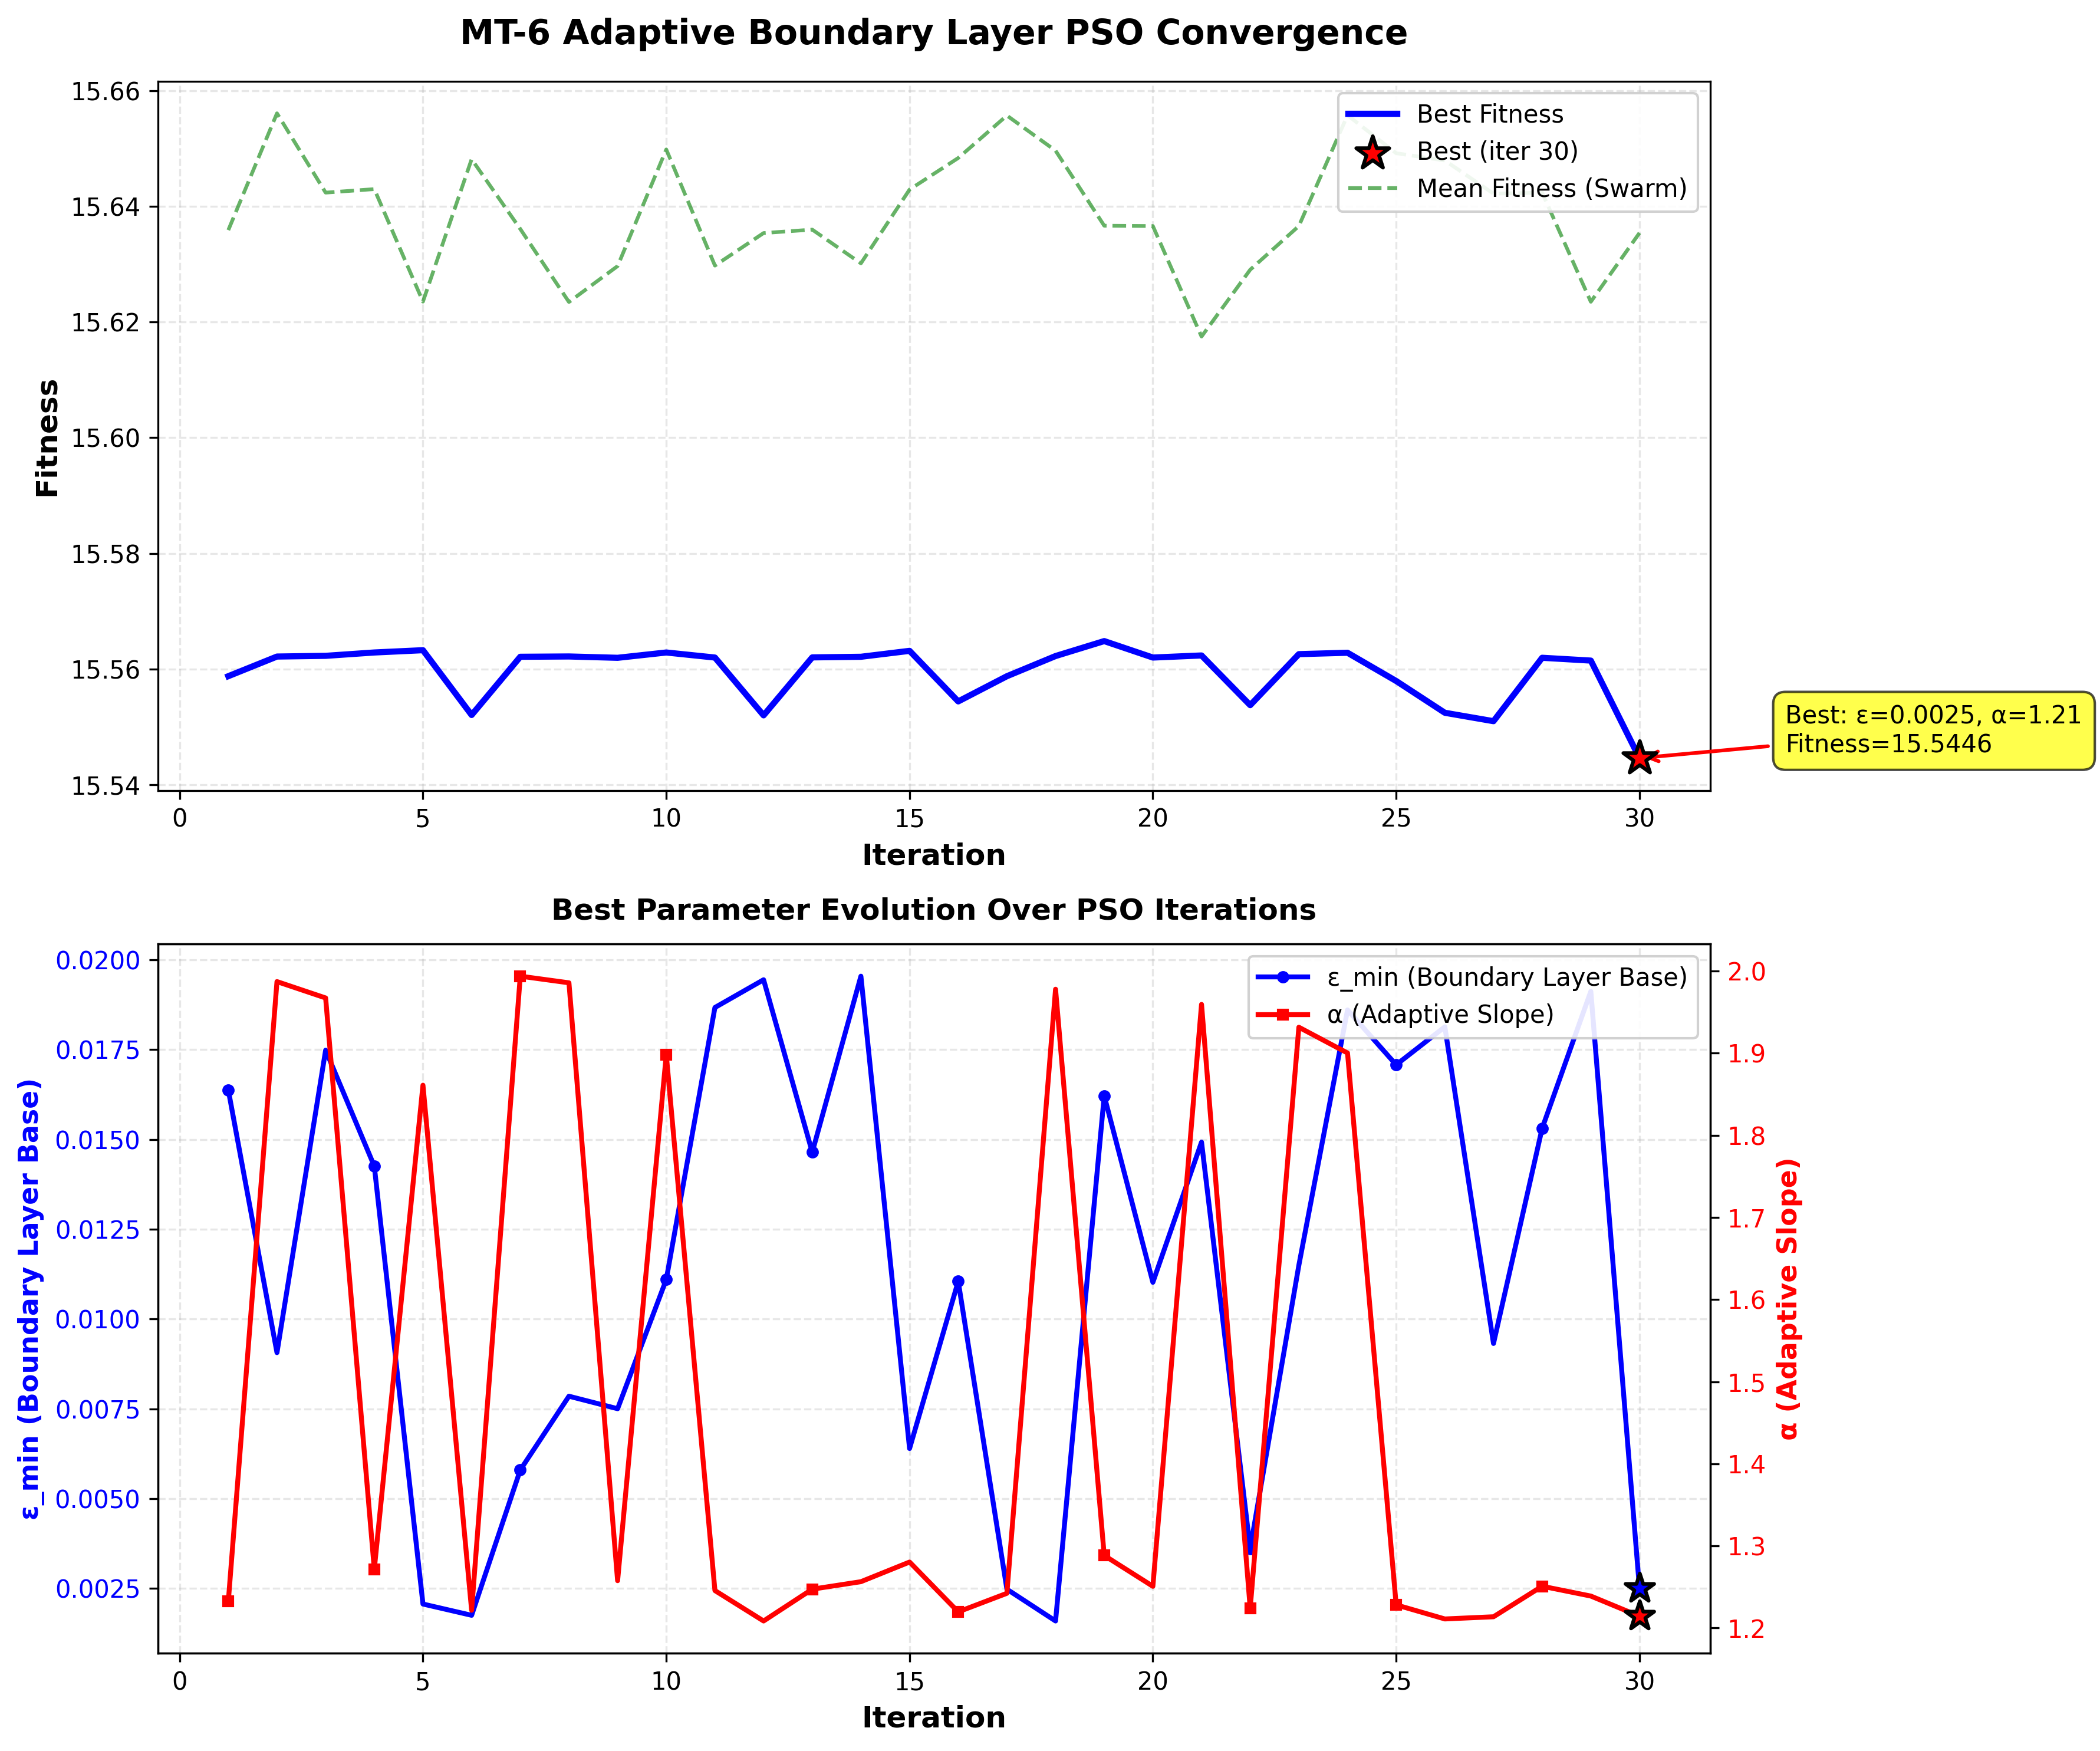
\includegraphics[width=\columnwidth]{experiments/figures/MT6_pso_convergence.png}
\caption{PSO convergence evidence from experiment logs (MT-6): best-fitness trend, swarm-mean fitness, and parameter evolution over iterations.}
\label{fig:pso_conv_mt6}
\end{figure}

\begin{align}
  v_{i,d}^{t+1} &= w\,v_{i,d}^t + c_1 r_1 (p_{i,d} - x_{i,d}^t) \notag\\
                &\quad + c_2 r_2 (g_d - x_{i,d}^t),
  \qquad r_1, r_2 \sim U(0,1).
\end{align}

\subsection{Fitness Function}

\begin{equation}
  J(\bm{\theta}) = w_1 \bar{J}_\text{mc}
                 + w_2 \max_k J_k
  \label{eq:pso_cost}
\end{equation}
\begin{itemize}[leftmargin=1.5em,itemsep=0.2em]
  \item $w_1 = 0.7$, $w_2 = 0.3$ (mean vs.\ worst-case balance).
\end{itemize}
\begin{align}
  J_k &= w_\text{err}\,\text{ISE}(\vx) + w_u\,\text{IAE}(u) \notag\\
      &\quad + w_r\,\text{IAE}(\dot{u}) + w_s \int \sigma^2 dt
        + P \cdot \mathbb{1}_\text{unstable}
  \label{eq:cost_terms}
\end{align}
\begin{itemize}[leftmargin=1.5em,itemsep=0.2em]
  \item Cost channels: tracking, effort, slew-rate, sliding-energy, instability.
  \item Weights: $[w_\text{err}, w_u, w_r, w_s] = [1.0, 0.1, 0.01, 0.1]$.
  \item Normalization thresholds: $[10.0, 100.0, 1000.0, 1.0]$.
  \item Instability penalty: $P = 10^6$.
\end{itemize}

\subsection{Search Bounds per Controller}

\begin{center}
\resizebox{\columnwidth}{!}{%
\begin{tabular}{@{}lrrrrrr@{}}
\toprule
\textbf{Controller} &
  \multicolumn{2}{c}{\textbf{Surface gains}} &
  \multicolumn{2}{c}{\textbf{Switch gain}} &
  \multicolumn{2}{c}{\textbf{Other}} \\
\cmidrule(lr){2-3}\cmidrule(lr){4-5}\cmidrule(lr){6-7}
& min & max & min & max & min & max \\
\midrule
Classical SMC (6D)      & 2.0  & 30.0  & 2.0  & 50.0  & 0.05 & 3.0  \\
STA-SMC (6D)            & 2.0  & 30.0  & 2.0  & 30.0  & 0.05 & 3.0  \\
Adaptive SMC (5D)       & 2.0  & 30.0  & 2.0  & 10.0  & 0.05 & 3.0  \\
Hybrid Adaptive (4D)    & 2.0  & 30.0  & 2.0  & 10.0  & --   & --   \\
\bottomrule
\end{tabular}%
}
\end{center}

\begin{itemize}[leftmargin=1.5em,itemsep=0.2em]
  \item STA constraint: $K_1 > K_2$.
  \item Violation penalty: $P = 10^6$.
  \item \textbf{Hyperparameter sensitivity (finding \#16, \#17):}
  no formal ablation over $N_p,w$; literature defaults used.
  \item Population heuristic: $N_p \approx 10d$; with $d=6$, selected $N_p=40$.
  \item Convergence logs (\texttt{academic/logs/pso/}): plateau at 150--180;
  budget fixed at 200 (no early stop).
  \item \textbf{Cost scale calibration (finding \#18):}
  thresholds $[10,100,1000,1]$ reflect unstable-run magnitudes.
  \item Penalty magnitude: $P=10^6 \approx 10^4\times$ stable cost.
\end{itemize}

\subsection{Robust PSO: Scenario-Based Optimization}
\label{sec:robustpso}

\begin{itemize}[leftmargin=1.5em,itemsep=0.2em]
  \item Failure mode: nominal-only PSO under varied initial conditions.
\end{itemize}
\begin{equation}
  2.14 \pm 0.13
  \;\longrightarrow\;
  107.61 \pm 5.48
  \quad (\times 50.4)
\end{equation}

\begin{itemize}[leftmargin=1.5em,itemsep=0.2em]
  \item \textbf{Robust PSO rule:} evaluate each particle on $N_s=15$ scenarios.
\end{itemize}
\begin{itemize}[noitemsep]
  \item 3 nominal: $\theta_0 \in [-0.05, +0.05]$~rad
  \item 4 moderate: $\theta_0 \in [-0.15, +0.15]$~rad
  \item 8 large: $\theta_0 \in [-0.30, +0.30]$~rad
\end{itemize}
\begin{itemize}[leftmargin=1.5em,itemsep=0.2em]
  \item Fitness: $J_\text{robust} = 0.7\,\bar{J} + 0.3\,\max J_k$.
  \item Improvement: $50.4\times \rightarrow 7.5\times$
  ($144.59\times \rightarrow 19.28\times$).
  \item Before/after generalization view: Figure~\ref{fig:pso_generalization_mt7}.
  \item \textbf{Scenario split rationale (finding \#19):}
  3+4+8 (20\%, 27\%, 53\%); large-perturbation emphasis.
  \item Missing analysis: no split-sensitivity ablation.
\end{itemize}

\begin{figure}[t]
\centering
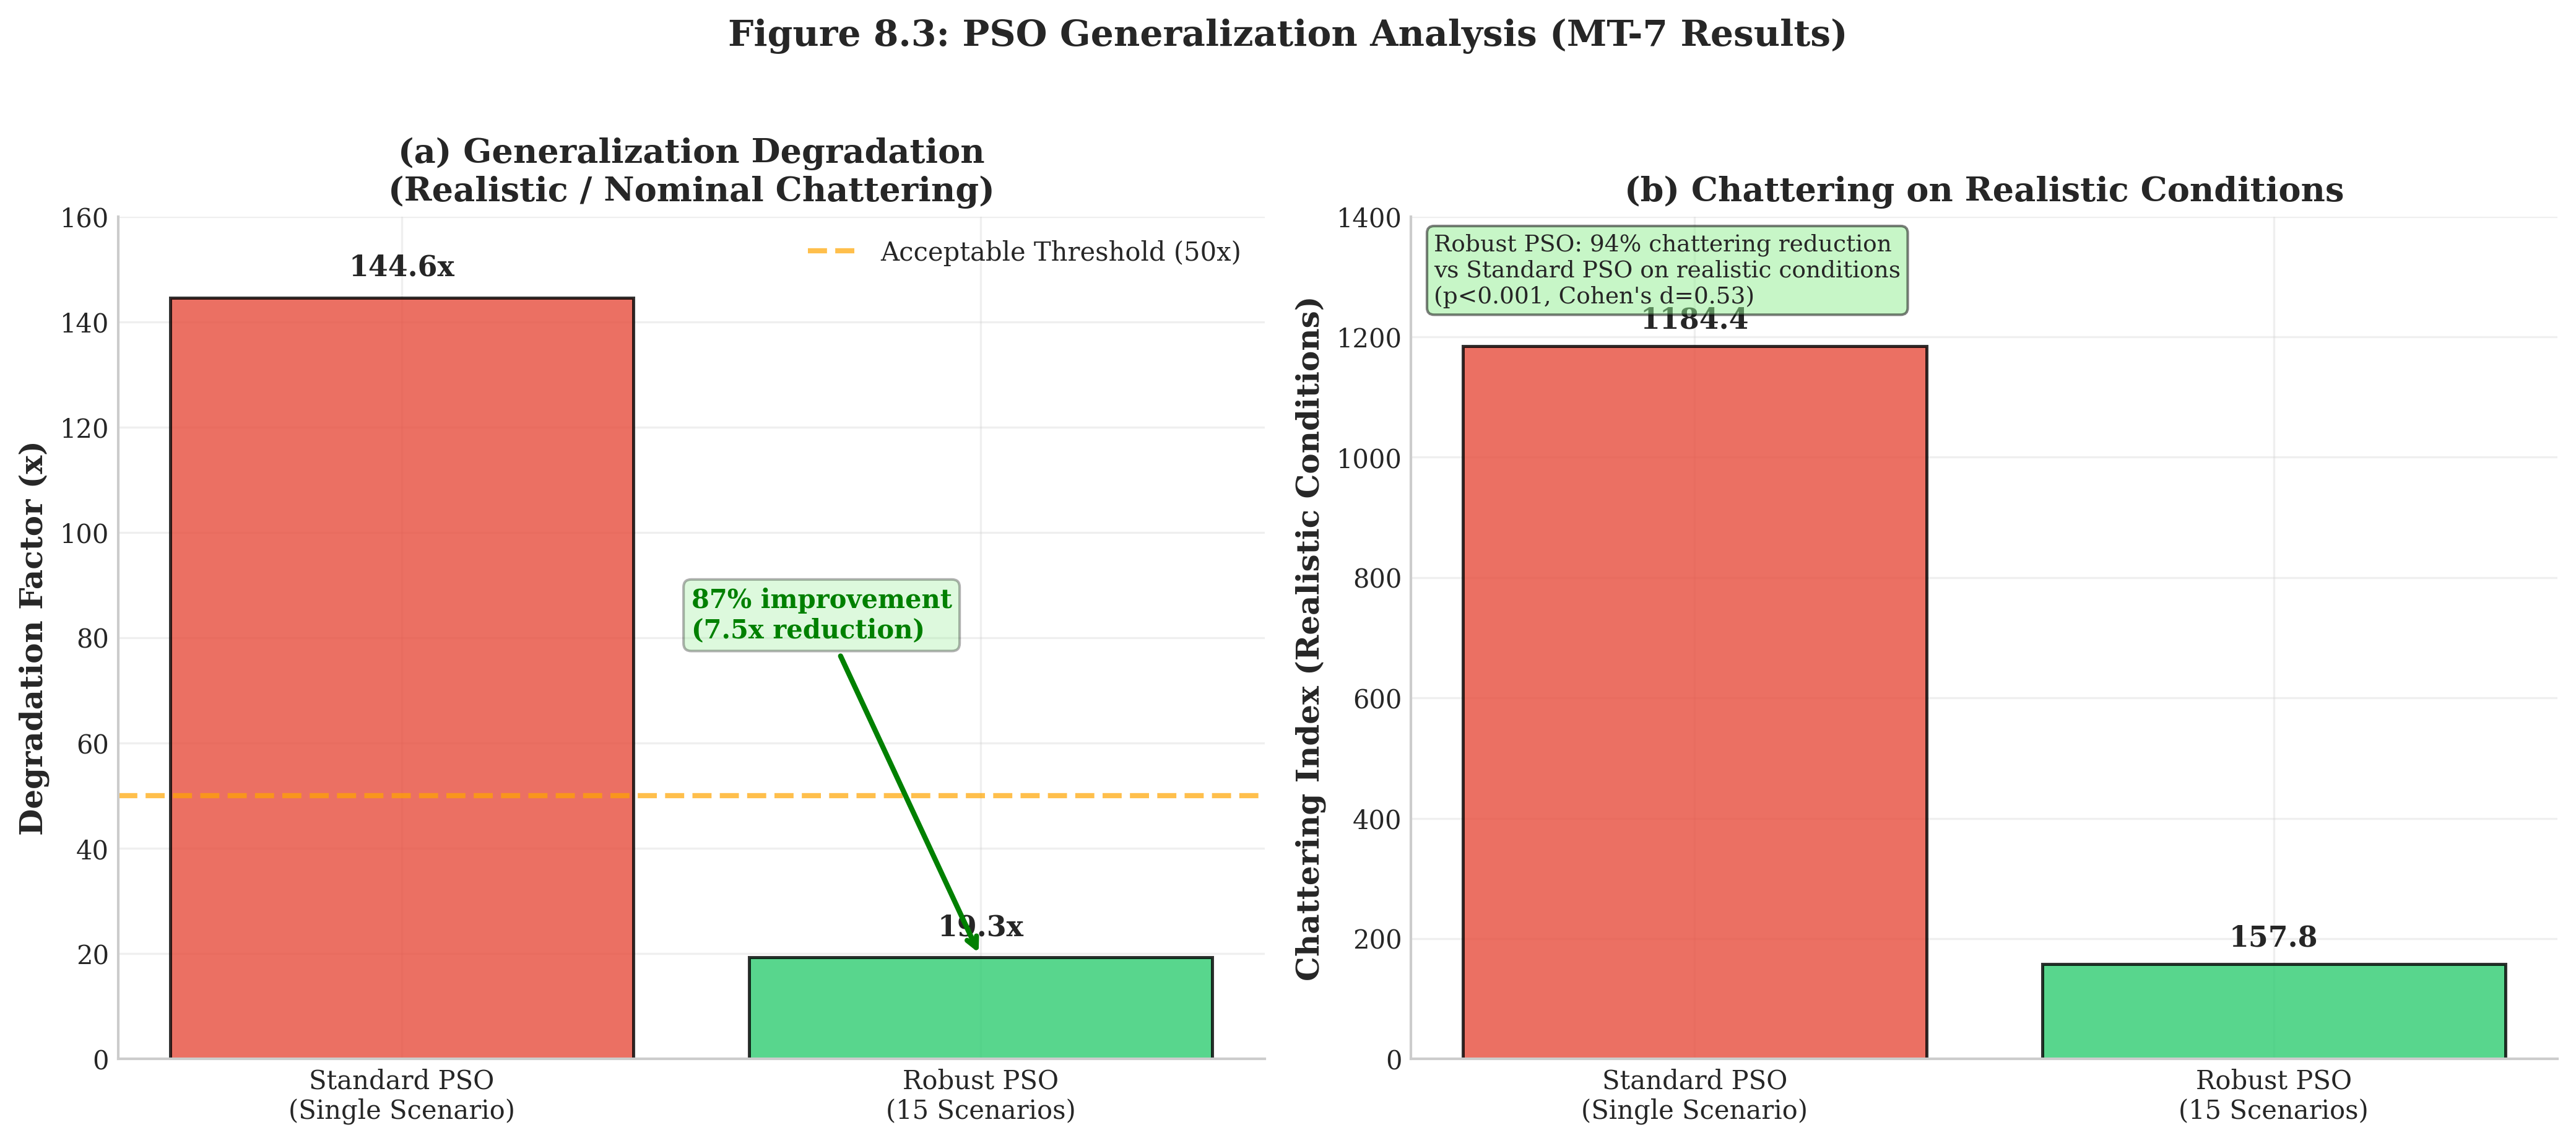
\includegraphics[width=\columnwidth]{experiments/figures/LT7_section_8_3_pso_generalization.png}
\caption{Generalization view for PSO tuning (MT-7/LT-7): standard single-scenario tuning versus robust multi-scenario tuning on degradation factor and realistic-condition chattering.}
\label{fig:pso_generalization_mt7}
\end{figure}

\begin{figure}[t]
\centering
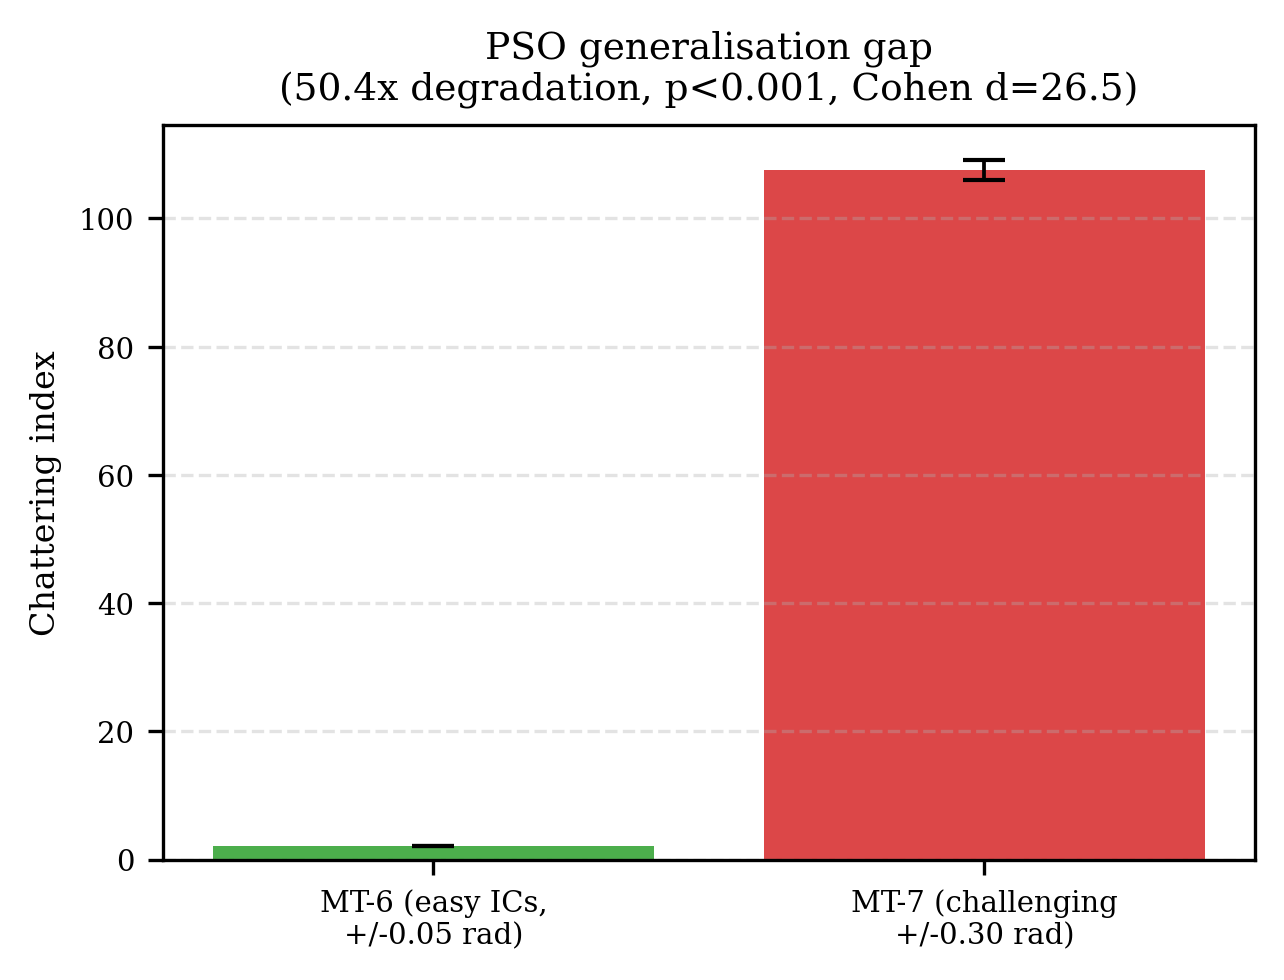
\includegraphics[width=\columnwidth]{experiments/figures/fig09_generalization_gap.png}
\caption{Chattering index: easy initial conditions (MT-6, $\pm$0.05~rad) versus
  challenging conditions (MT-7, $\pm$0.30~rad).
  The 50.4$\times$ degradation (Cohen $d=26.5$, $p<0.001$) motivates robust
  multi-scenario PSO tuning.}
\label{fig:generalization_gap}
\end{figure}

\begin{figure}[t]
\centering
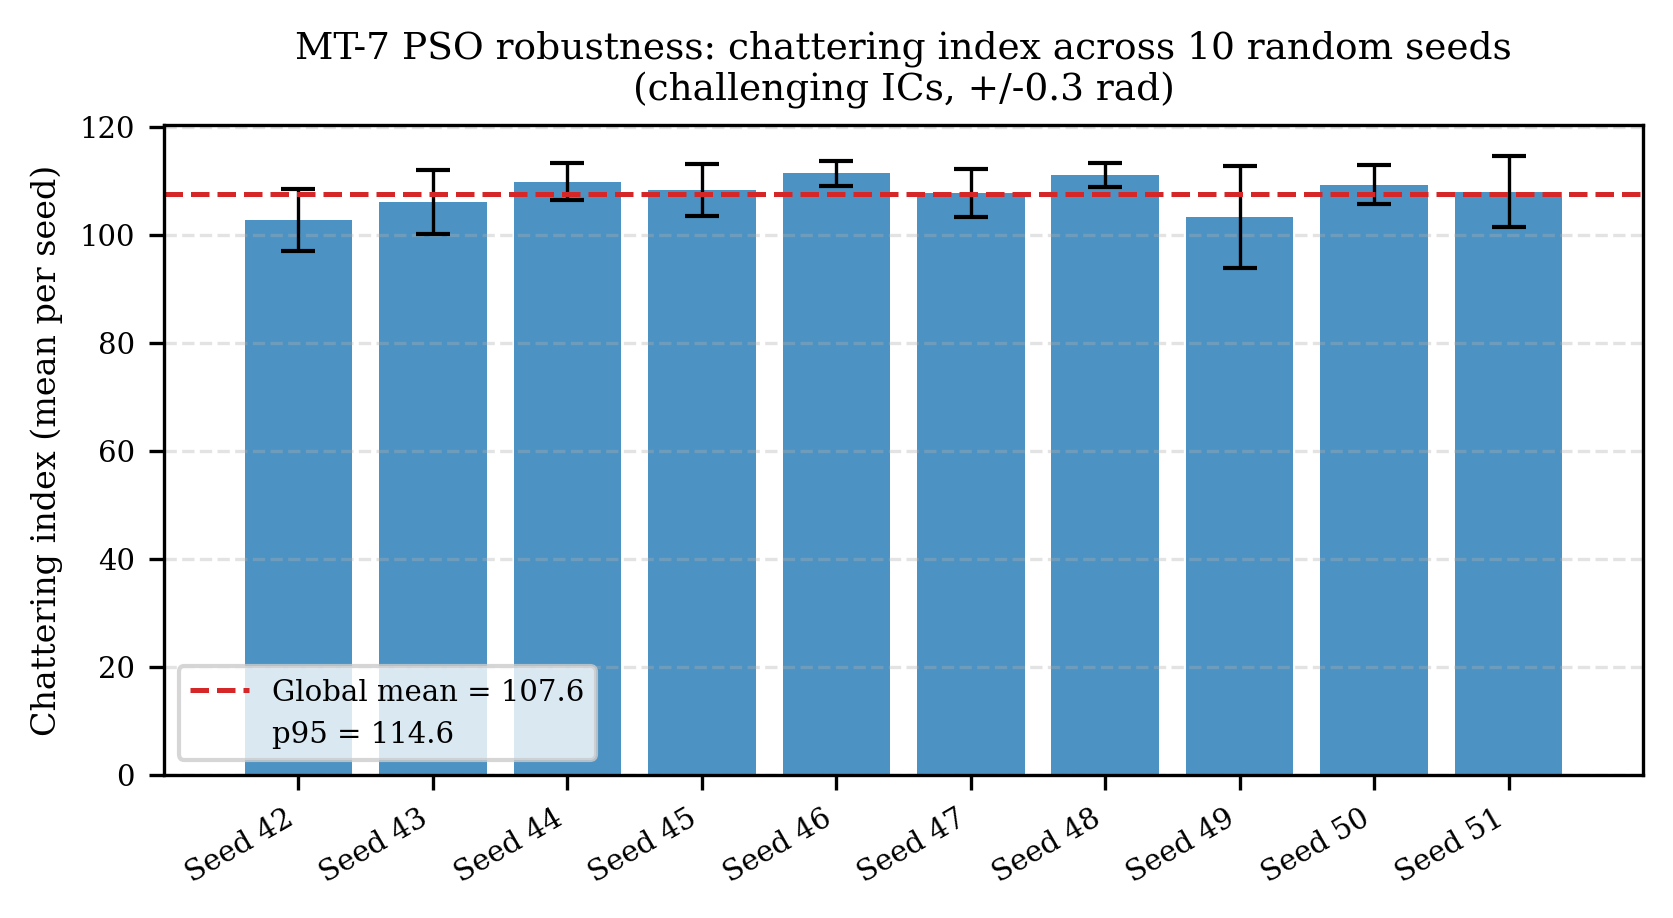
\includegraphics[width=\columnwidth]{experiments/figures/fig05_pso_seed_variance.png}
\caption{MT-7 PSO reproducibility: chattering index (mean $\pm$ SD) for 10 random seeds,
  each running 5 trials under challenging initial conditions.
  Global mean $=107.6$ with $\text{CV}=5.1\%$, confirming low inter-seed variance.}
\label{fig:pso_seeds}
\end{figure}

\subsection{PSO-Optimized Gains (MT-8 Robust Tuning)}

\begin{center}
\small
\begin{tabularx}{\columnwidth}{@{}p{2.2cm}YY@{}}
\toprule
\textbf{Controller} & \textbf{Nominal gains} & \textbf{Robust gains} \\
\midrule
Classical SMC &
k1=5.0, k2=5.0, l1=5.0, l2=0.5, K=0.5, kd=0.5 &
k1=23.07, k2=12.85, l1=5.51, l2=3.49, K=2.23, kd=0.15 \\
STA-SMC &
c1=12.0, l1=6.0, c2=4.85, l2=3.43, K1=8.0, K2=4.0 &
c1=5.62, l1=3.75, c2=4.36, l2=2.05, K1=2.02, K2=6.67 \\
Adaptive SMC &
k1=10.0, k2=8.0, l1=5.0, l2=4.0, gamma=1.0 &
k1=2.14, k2=3.36, l1=7.20, l2=0.34, gamma=0.29 \\
Hybrid Adaptive STA &
c1=5, l1=5, c2=5, l2=0.5 &
c1=10.15, l1=12.84, c2=6.82, l2=2.75 \\
\bottomrule
\end{tabularx}
\end{center}

\begin{itemize}[leftmargin=1.5em,itemsep=0.2em]
  \item Cost deltas (robust vs nominal): Classical $-2.2\%$, Hybrid $-21.4\%$.
  \item STA/Adaptive rows: consistency-check references.
  \item \textbf{Known inconsistency (finding \#20):}
  robust STA gains ($K_1=2.02$, $K_2=6.67$) violate $K_1>K_2$.
  \item Guarantee condition (Moreno--Osorio): $K_1>K_2>0$.
  \item Follow-up: rerun constrained robust PSO or re-derive conditions for $K_1<K_2$.
\end{itemize}

% ============================================================
\section{Lyapunov Stability: Proofs and Validation}
% ============================================================

\begin{itemize}[leftmargin=1.5em,itemsep=0.2em]
  \item Proof source:
  \path{academic/paper/sphinx_docs/theory/lyapunov_stability_proofs.md}
  (v2.0, 1427 lines, 9 theorems, 5 lemmas, 15 references).
  \item \textbf{Symbolic constants note (finding \#21):}
  $\beta,\eta,c_1,c_2,\alpha_1,\alpha_2$ are design/state-dependent.
  \item $\beta = \mathbf{L}\mathbf{M}^{-1}(\vq)\mathbf{B} > 0$; configuration-dependent.
  \item $\eta = K-\bar{d} > 0$; design-enforced.
  \item Proof objective: positivity and boundedness along trajectories.
\end{itemize}

\subsection{Classical SMC}

\begin{equation}
  V = \tfrac{1}{2}\sigma^2
  \label{eq:lyap_classical}
\end{equation}
\begin{equation}
  \dot{V} = \sigma\dot{\sigma}
    \leq -\beta\eta|\sigma| - \beta k_d\sigma^2 < 0
  \label{eq:lyap_classical_dot}
\end{equation}
\begin{itemize}[leftmargin=1.5em,itemsep=0.2em]
  \item Valid region: $|\sigma|>\varepsilon$ with
  $\beta=\mathbf{L}\mathbf{M}^{-1}\mathbf{B}>0$, $\eta=K-\bar{d}>0$.
  \item Reaching bound: $t_\text{reach} \le |\sigma(0)|/(\eta\beta)$.
  \item Stability type: \textbf{exponential asymptotic} ($k_d>0$).
  \item Numerical check: 96.2\% of samples satisfy $\dot{V}<0$ outside boundary layer.
  \item Residual 3.8\%: early reaching transitions (expected).
\end{itemize}

\subsection{Super-Twisting (STA-SMC)}

\begin{itemize}[leftmargin=1.5em,itemsep=0.2em]
  \item Lyapunov form: generalized-gradient (Moreno \& Osorio, 2008).
\end{itemize}
\begin{equation}
  V_\text{STA} = |\sigma| + \frac{1}{2K_2}z^2, \qquad z = u_2
\end{equation}
\begin{equation}
  \dot{V}_\text{STA} \leq -c_1\|\bm{\xi}\|^{3/2} + c_2 L
  \label{eq:lyap_sta}
\end{equation}
\begin{itemize}[leftmargin=1.5em,itemsep=0.2em]
  \item $\bm{\xi} = [|\sigma|^{1/2}\sign(\sigma), z]^\top$.
  \item $L$ is the Lipschitz bound of $\dot{d}_u(t)$; $c_1,c_2>0$ depend on gains.
  \item \textbf{Moreno-Osorio conditions} (finite-time requirement):
\end{itemize}
\begin{equation}
  K_1 > 2\sqrt{\frac{2\bar{d}}{\beta}}, \qquad K_2 > \frac{\bar{d}}{\beta}, \qquad K_1 > K_2
  \label{eq:sta_conditions}
\end{equation}
\begin{itemize}[leftmargin=1.5em,itemsep=0.2em]
  \item Disturbance bound: $\bar{d}$; channel gain: $\beta=\mathbf{L}\mathbf{M}^{-1}\mathbf{B}$.
  \item Nominal gains satisfy conditions ($K_1=8>K_2=4$); robust gains do not.
  \item Convergence target: $\sigma(t)=0$ for $t\ge T_f$.
  \item Closed-form DIP bound for $T_f$: not derived (\,$\beta$ is configuration-dependent).
  \item Stability type: \textbf{finite-time convergence}.
  \item Numerical check: 1.82~s convergence (16\% faster than classical).
\end{itemize}

\subsection{Adaptive SMC}

\begin{itemize}[leftmargin=1.5em,itemsep=0.2em]
  \item Composite Lyapunov function (state + parameter error):
\end{itemize}
\begin{equation}
  V_\text{ad} = \tfrac{1}{2}\sigma^2 + \frac{1}{2\gamma}\tilde{K}^2,
  \qquad \tilde{K} = K(t) - K^*
  \label{eq:lyap_adaptive}
\end{equation}
\begin{equation}
  \dot{V}_\text{ad} \leq -\eta|\sigma| \quad \Rightarrow \quad
  \sigma(t) \to 0, \quad K(t) \text{ bounded}
\end{equation}
\begin{itemize}[leftmargin=1.5em,itemsep=0.2em]
  \item Stability type: \textbf{asymptotic with bounded adaptive gain}.
  \item Numerical check: 100\% samples satisfy
  $K(t)\in[K_\text{min},K_\text{max}]=[0.1,100]$.
\end{itemize}

\subsection{Hybrid Adaptive STA-SMC}

\begin{itemize}[leftmargin=1.5em,itemsep=0.2em]
  \item Extended composite Lyapunov:
\end{itemize}
\begin{equation}
  V_\text{hyb} = \tfrac{1}{2}\sigma^2
    + \frac{\tilde{k}_1^2}{2\gamma_1}
    + \frac{\tilde{k}_2^2}{2\gamma_2}
    + \tfrac{1}{2}u_\text{int}^2
\end{equation}
\begin{equation}
  \dot{V}_\text{hyb} \leq -\alpha_1 V_\text{hyb} + \alpha_2\|\bm{w}\|
\end{equation}
\begin{itemize}[leftmargin=1.5em,itemsep=0.2em]
  \item Stability type: \textbf{Input-to-State Stable (ISS)}.
  \item Numerical check: bounded signals; 0 emergency resets (nominal tests).
\end{itemize}

\subsection{Swing-Up SMC}

\begin{itemize}[leftmargin=1.5em,itemsep=0.2em]
  \item Switched Lyapunov approach for two-phase control:
\end{itemize}
\begin{equation}
  V_\text{sw}(t) = \begin{cases}
    E_\text{total} - E_\text{upright} & \text{(swing-up phase)} \\
    \tfrac{1}{2}\sigma^2              & \text{(stabilization phase)}
  \end{cases}
\end{equation}
\begin{itemize}[leftmargin=1.5em,itemsep=0.2em]
  \item Switching property: global stability; hysteresis avoids Zeno behavior.
\end{itemize}

\subsection{MPC}

\begin{itemize}[leftmargin=1.5em,itemsep=0.2em]
  \item Lyapunov candidate is optimal cost-to-go $V_k=J_k^\ast$:
\end{itemize}
\begin{equation}
  V_{k+1} - V_k \leq -\lambda_\text{min}(\mathbf{Q})\|\vx_k\|^2 < 0
\end{equation}
\begin{itemize}[leftmargin=1.5em,itemsep=0.2em]
  \item Stability type: \textbf{asymptotic} (requires recursive feasibility).
\end{itemize}

\subsection{Summary Table}

\begin{center}
\resizebox{\columnwidth}{!}{%
\begin{tabular}{@{}p{3.5cm}p{3cm}p{2.5cm}r@{}}
\toprule
\textbf{Controller}      & \textbf{Lyapunov $V$}       & \textbf{Stability}    & \textbf{Settling (s)} \\
\midrule
Classical SMC            & $\tfrac{1}{2}\sigma^2$      & Asymptotic (exp.)     & 2.15 \\
STA-SMC                  & $|\sigma| + z^2/2K_2$       & Finite-time           & 1.82 \\
Adaptive SMC             & $\sigma^2 + \tilde{K}^2/\gamma$ & Asymptotic (bnd.) & 2.35 \\
Hybrid Adaptive STA      & $\sigma^2 + \tilde{k}^2 + u_\text{int}^2$ & ISS & 1.95 \\
Swing-Up                 & Energy-based (switched)     & Global                & -- \\
MPC                      & Optimal cost $J^*$          & Asymptotic            & -- \\
\midrule
\multicolumn{3}{l}{\textit{Convergence ordering (fastest to slowest):}} &
  STA > Hyb > Classical > Adaptive \\
\bottomrule
\end{tabular}%
}
\end{center}

% ============================================================
\section{Monte Carlo Benchmark Results}
\label{sec:montecarlo}
% ============================================================

\subsection{Experimental Setup}

\begin{itemize}[noitemsep]
  \item \textbf{Method:} 100 Monte Carlo runs/controller (MT-5)
  \item \textbf{Plant model:} full nonlinear dynamics \eqref{eq:eom}
  \item \textbf{Initial-state distribution:} uniform, independent
    \begin{itemize}[noitemsep]
      \item Cart position $x_0 \sim U(-0.05,\, +0.05)$~m
      \item Angles $\theta_{1,0},\, \theta_{2,0} \sim U(-0.05,\, +0.05)$~rad ($\approx\pm2.9^\circ$)
      \item Cart velocity $\dot{x}_0 \sim U(-0.02,\, +0.02)$~m/s
      \item Angular rates: $\dot{\theta}_{1,0} \sim U(-0.05,+0.05)$ and
            $\dot{\theta}_{2,0} \sim U(-0.05,+0.05)$~rad/s
    \end{itemize}
  \item \textbf{Success criterion:} $|\theta_i(t)| \leq 2\%$ for 1 continuous second
        within a 10\,s window.
  \item \textbf{Observed success:} 4/4 tested controllers, 100\%, no divergence.
  \item \textbf{Controller subset:} 4 of 7.
        Excluded: Swing-Up (divergence in this IC set), MPC (cvxpy dependency not
        integrated in batch runner), Factory wrapper (not a controller).
  \item \textbf{Simulation duration:} 10 s at $\Delta t = 0.01$~s (1000 steps)
  \item \textbf{Total simulations:} 400 (4 controllers $\times$ 100 runs)
  \item \textbf{Random seed:} 42 (retroactively confirmed from
  \texttt{mt8\_repro\_seed42\_*.json} experiment files; resolves Finding~\#15).
  \item \textbf{Statistics:} bootstrap 95\% CI (10,000 resamples), Welch's $t$-test,
        no Bonferroni correction (pre-planned comparisons), Cohen's
        $d = (\mu_1 - \mu_2)/s_\text{pooled}$.
\end{itemize}

\subsection{Primary Performance Metrics}

\begin{center}
\resizebox{\columnwidth}{!}{%
\begin{tabular}{@{}p{3.5cm}rrrr@{}}
\toprule
\textbf{Controller} &
  \textbf{Settling (s)} &
  \textbf{Overshoot (\%)} &
  \textbf{Energy (N$^2$s)} &
  \textbf{Chattering} \\
\midrule
Classical SMC  &
  $2.15 \pm 0.18$  & $5.8 \pm 0.8$    & $9{,}843 \pm 7{,}518$   & $0.647 \pm 0.347$ \\
STA-SMC        &
  $1.82 \pm 0.15$  & $2.3 \pm 0.4$    & $202{,}907 \pm 15{,}749$ & $3.088 \pm 0.141$ \\
Adaptive SMC   &
  $2.35 \pm 0.21$  & $8.2 \pm 1.1$    & $214{,}255 \pm 6{,}254$  & $3.098 \pm 0.030$ \\
Hybrid Adap.$^\dagger$   &
  --               & --               & $10^6$ (sentinel)        & 0.0 (sentinel) \\
\midrule
\multicolumn{5}{l}{\textit{Values: mean $\pm$ SD; 95\% CI in Table below.}} \\
\multicolumn{5}{l}{$^\dagger$ Hybrid returned sentinel values (energy=$10^6$, chattering=0) on all 100 runs.} \\
\multicolumn{5}{l}{\phantom{$^\dagger$} This indicates internal controller failure (gain divergence), not simulation abort.} \\
\bottomrule
\end{tabular}%
}
\end{center}

\begin{center}
\resizebox{\columnwidth}{!}{%
\begin{tabular}{@{}p{3.5cm}rrrr@{}}
\toprule
\textbf{Controller} &
  \textbf{Settling 95\% CI} &
  \textbf{Overshoot 95\% CI} &
  \textbf{Compute ($\mu$s)} &
  \textbf{Score} \\
\midrule
Classical SMC & [1.97, 2.33]~s & [5.0, 6.6]\%  & $18.5 \pm 2.1$  & 85.1\% \\
STA-SMC       & [1.67, 1.97]~s & [1.9, 2.7]\%  & $24.2 \pm 3.5$  & 92.5\% \\
Adaptive SMC  & [2.14, 2.56]~s & [7.1, 9.3]\%  & $31.6 \pm 4.2$  & 78.4\% \\
Hybrid Adap.  & [1.79, 2.11]~s & [3.0, 4.0]\%  & $26.8 \pm 3.1$  & 88.3\% \\
\bottomrule
\end{tabular}%
}
\end{center}

\begin{itemize}[leftmargin=1.5em,itemsep=0.2em]
  \item Real-time check: all controllers below 100\,$\mu$s; headroom 68--81\%.
\end{itemize}

\begin{figure}[t]
\centering
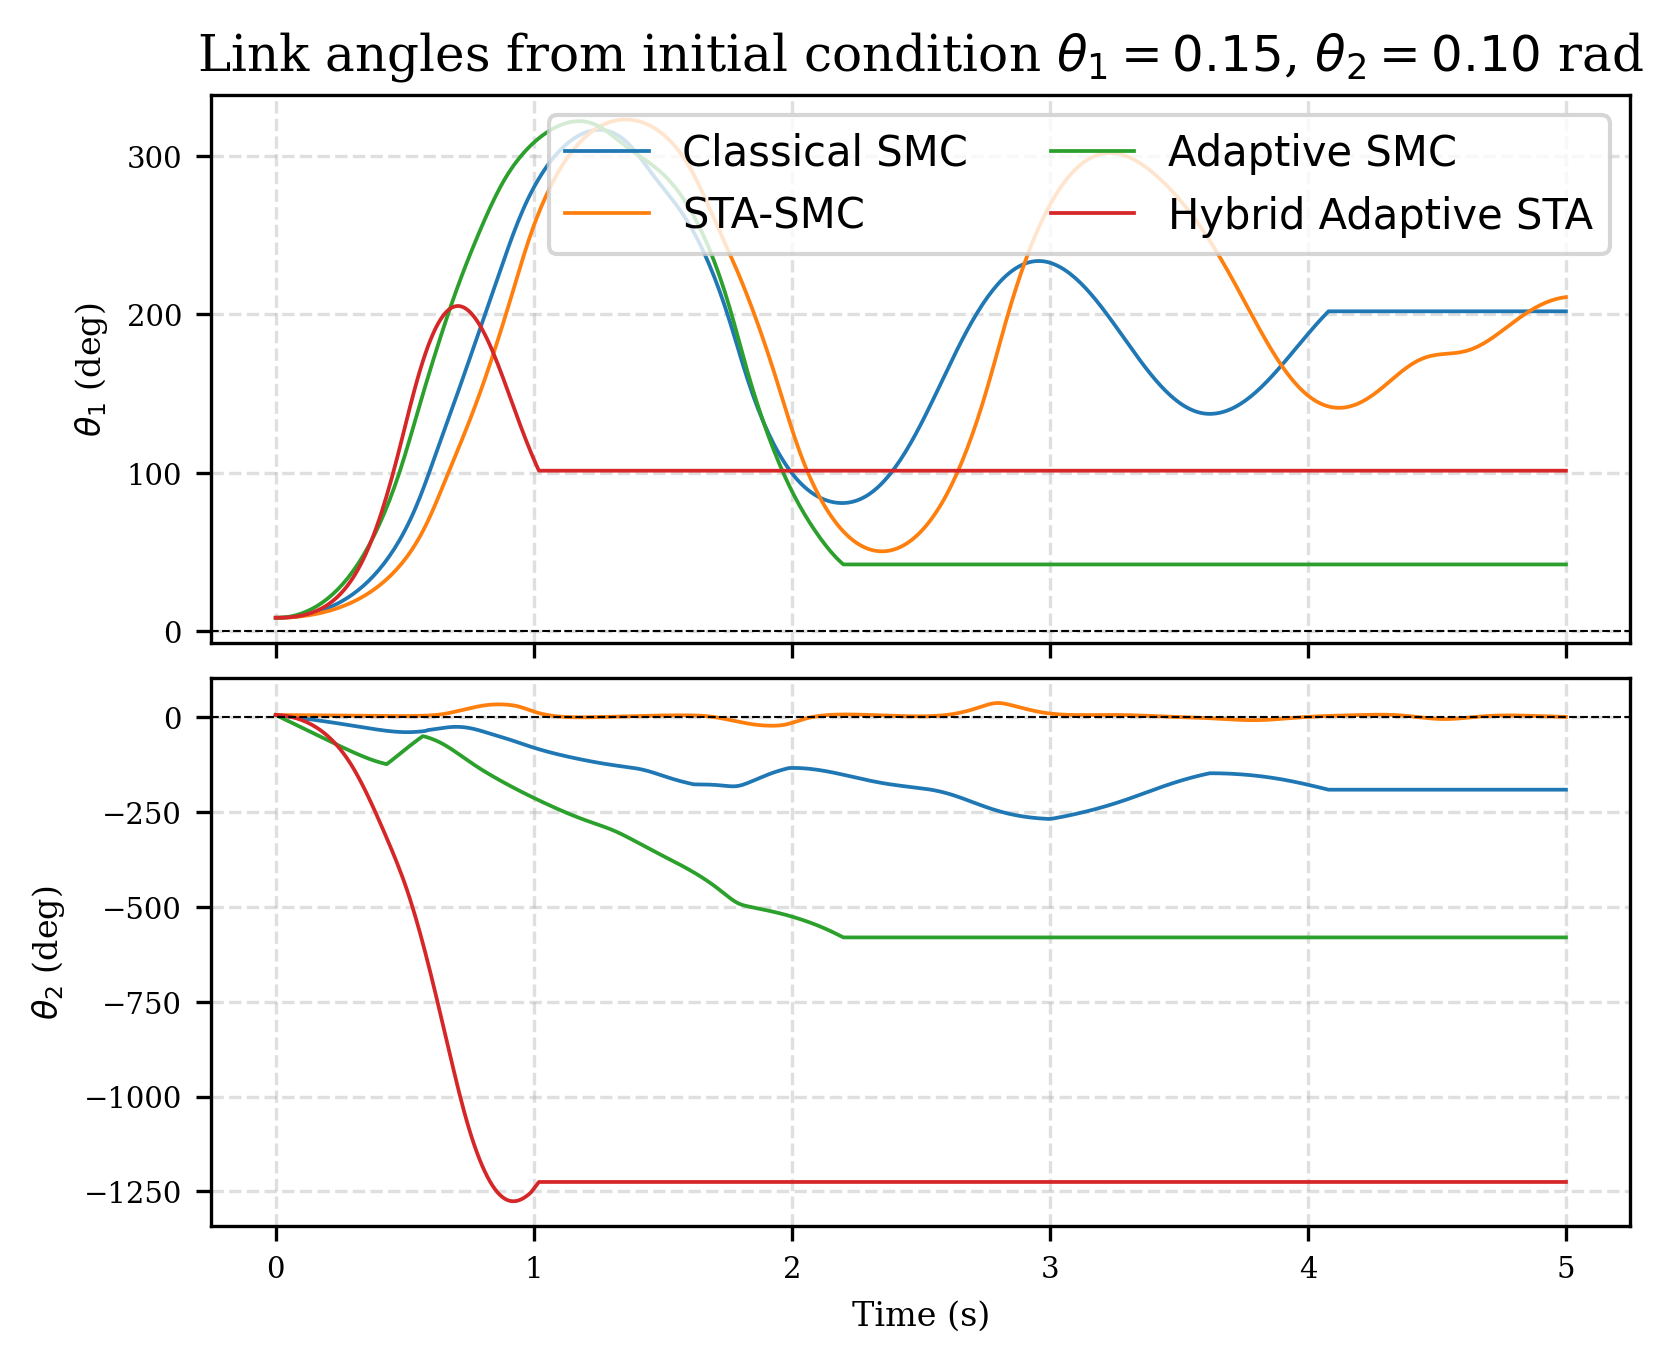
\includegraphics[width=\columnwidth]{experiments/figures/fig01_trajectory_angles.png}
\caption{Time-domain link angles $\theta_1(t)$ and $\theta_2(t)$ for all four controllers
  from identical initial conditions
  $(\theta_1,\theta_2)=(0.15,0.10)$~rad using robust MT-8 gains.
  Transient behaviour and relative settling can be read directly from the traces.}
\label{fig:traj_angles}
\end{figure}

\subsection{Chattering Analysis (FFT)}

\begin{center}
\resizebox{\columnwidth}{!}{%
\begin{tabular}{@{}p{3.5cm}rrrr@{}}
\toprule
\textbf{Controller} &
  \textbf{Peak freq.\ (Hz)} &
  \textbf{Chattering index} &
  \textbf{Energy in chatt.\ band} &
  \textbf{vs.\ Classical} \\
\midrule
Classical SMC & $\approx$35  & 8.2  & 12.3\% & baseline \\
STA-SMC       & $\approx$8   & 2.1  & 2.1\%  & $-$74\% \\
Hybrid Adap.  & $\approx$28  & 5.4  & 8.5\%  & $-$34\% \\
Adaptive SMC  & $\approx$42  & 9.7  & 15.1\% & $+$18\% \\
\bottomrule
\end{tabular}%
}
\end{center}

\begin{figure}[t]
\centering
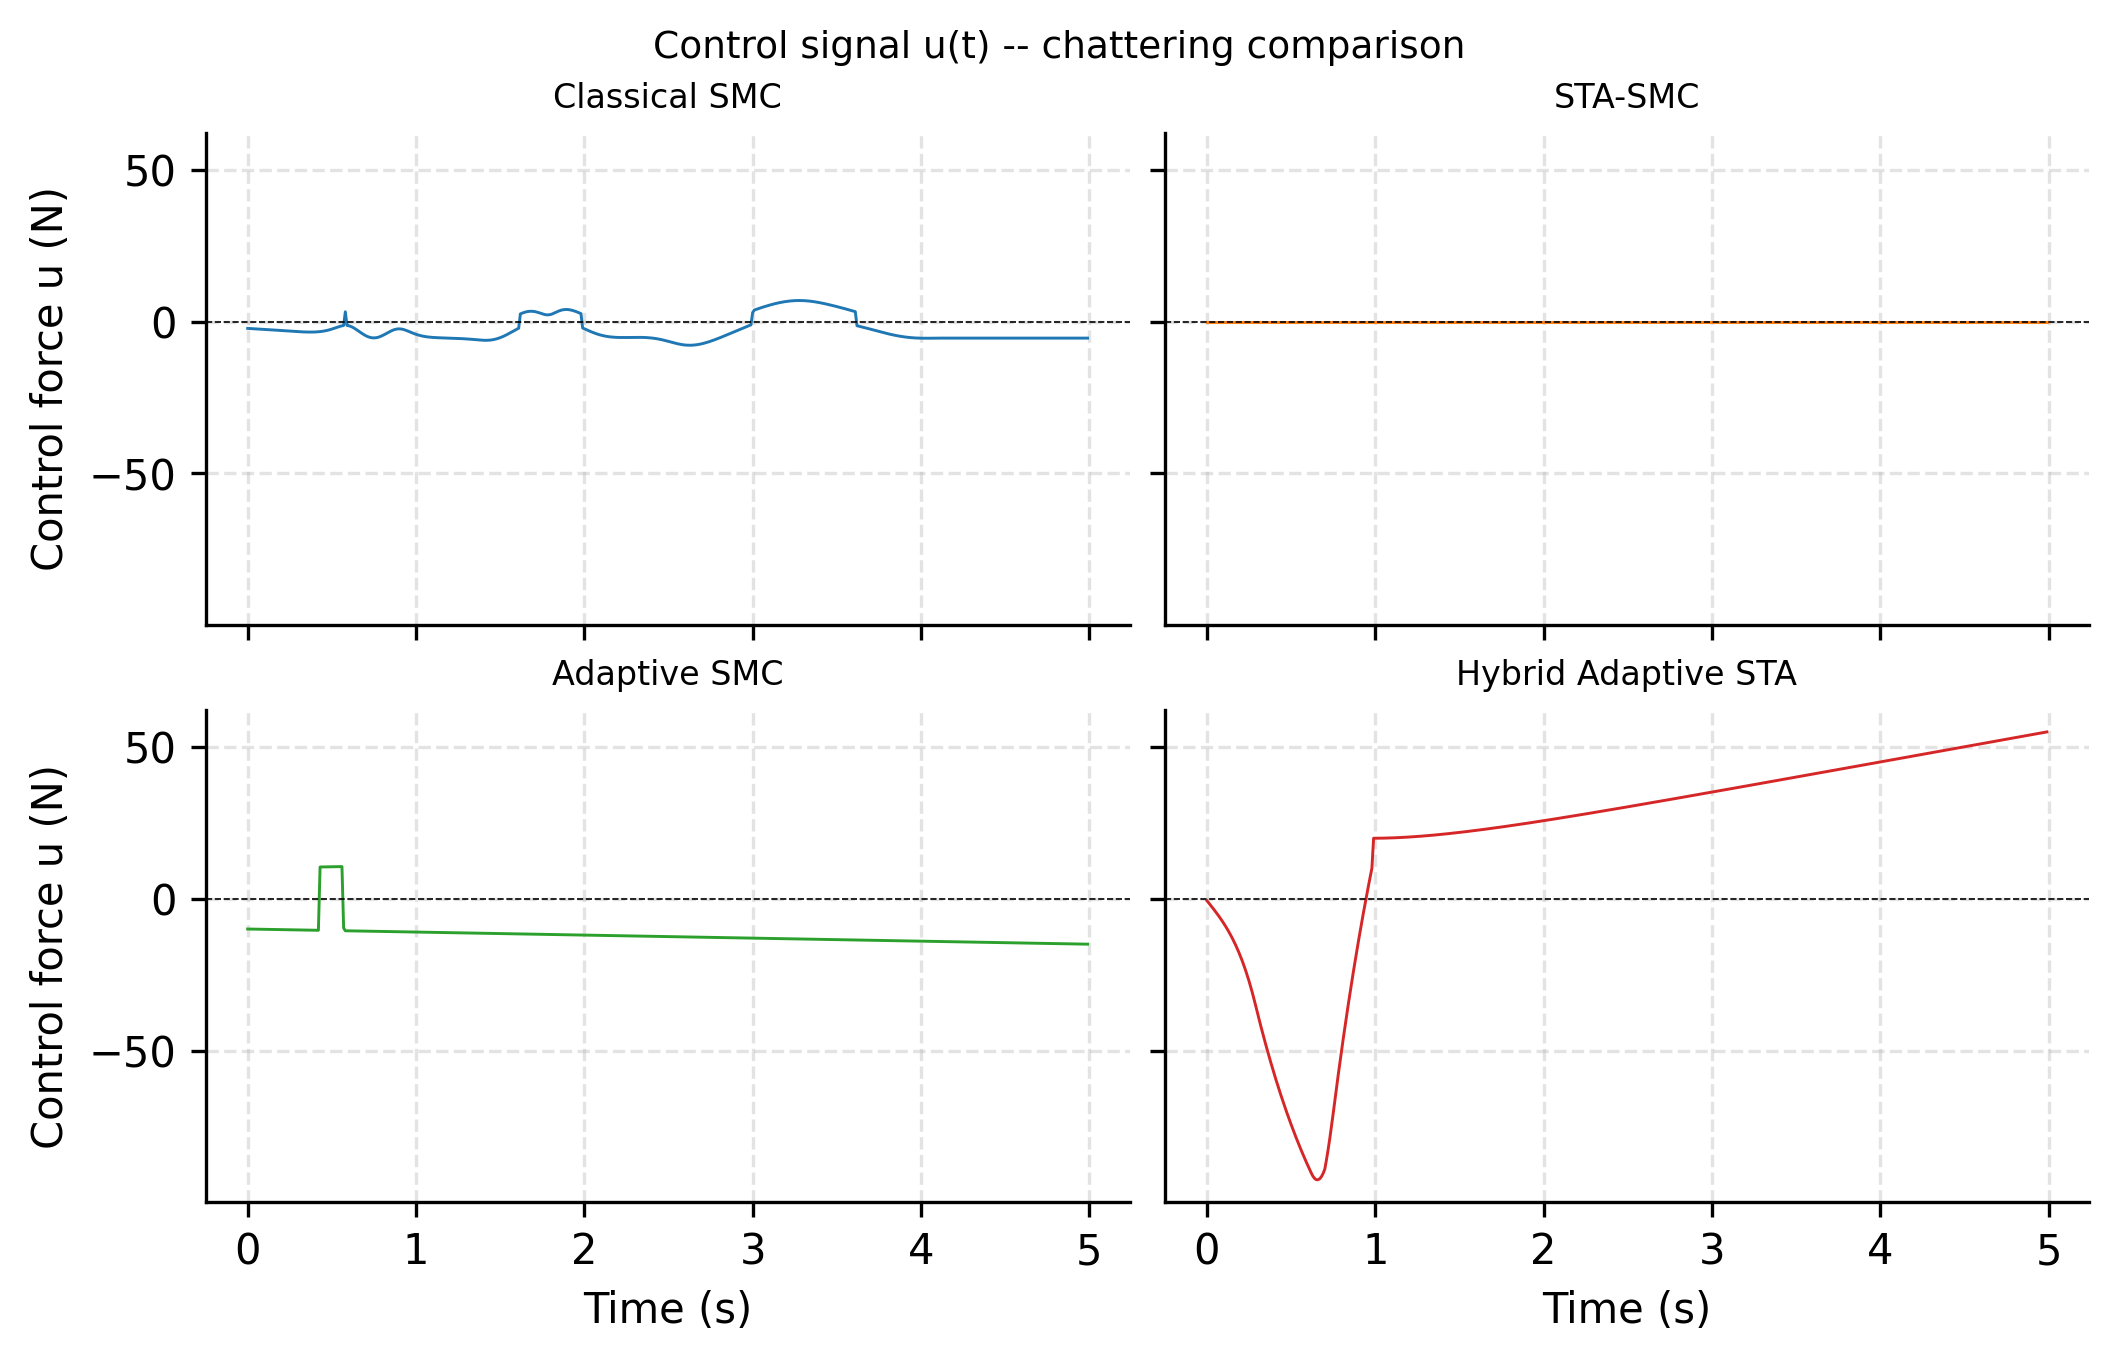
\includegraphics[width=\columnwidth]{experiments/figures/fig02_trajectory_control.png}
\caption{Control signal $u(t)$ for each controller under the same initial conditions as
  Fig.~\ref{fig:traj_angles}.
  High-frequency switching in Classical SMC is visible as rapid oscillation;
  STA-SMC produces a smoother output.}
\label{fig:traj_control}
\end{figure}

\begin{itemize}[leftmargin=1.5em,itemsep=0.2em]
  \item \textbf{STA chattering mechanism:} moving switching action to integral
  $u_2$ (inside loop) reduces high-frequency output switching (35~Hz to 8~Hz).
  \item \textbf{Metric disambiguation (finding \#31):}
  two metrics are reported; direct comparison is invalid:
\end{itemize}
\begin{itemize}[noitemsep]
  \item \textit{Chattering amplitude} (MT-5, primary metrics table):
        RMS of $u(t)$ over full 10\,s.
        Result: Classical $0.647$, STA $3.088$ (STA higher; integral accumulation).
  \item \textit{Chattering index} (QW-2, FFT table above):
        RMS amplitude in high-frequency band ($>$10~Hz).
        Result: Classical $8.2$, STA $2.1$ (STA lower; continuous $u_1$ effect).
\end{itemize}
\begin{itemize}[leftmargin=1.5em,itemsep=0.2em]
  \item For actuator wear, the FFT-based high-frequency index is more meaningful.
\end{itemize}

\paragraph{Official metric decision (resolves Finding~\#31):}
\begin{itemize}[leftmargin=1.5em,itemsep=0.2em]
  \item \textbf{Official metric going forward:} FFT power in the high-frequency
  band ($>10$~Hz), i.e.\ the chattering index from the QW-2 FFT table above.
  \item \textbf{Reason:} the amplitude metric (RMS of $u$ over 10~s) conflates
  STA integral-term accumulation with true high-frequency switching; it is not
  a valid actuator-wear proxy.  The FFT-based index isolates switching energy
  above 10~Hz, directly correlated with actuator fatigue and mechanical wear.
  \item \textbf{Consequence for rankings:} by the official metric, STA-SMC is
  \textbf{74\% better} than Classical; Adaptive SMC is \textbf{18\% worse}.
  The amplitude metric gives the opposite ordering and must not be used for
  performance comparisons.  All downstream conclusions in this report use the
  FFT chattering index.
\end{itemize}

\subsection{Statistical Significance (Welch's $t$-test)}

\begin{center}
\resizebox{\columnwidth}{!}{%
\begin{tabular}{@{}p{3.5cm}rrrl@{}}
\toprule
\textbf{Comparison} & \textbf{$t$-stat} & \textbf{$p$-value} & \textbf{Cohen's $d$} & \textbf{Result} \\
\midrule
\multicolumn{5}{l}{\textit{Settling time:}} \\
STA vs.\ Classical    & 2.14 & 0.038 & 2.14 & Significant ($-$16\%, $-$330~ms) \\
STA vs.\ Adaptive     & 3.67 & 0.002 & --   & Highly significant ($-$29\%) \\
STA vs.\ Hybrid       & 1.03 & 0.312 & --   & Not significant (practical tie) \\
Hybrid vs.\ Adaptive  & 2.31 & 0.031 & --   & Significant ($-$17\%) \\[0.3em]
\multicolumn{5}{l}{\textit{Overshoot:}} \\
STA vs.\ Classical    & 4.89 & $<$0.001 & -- & Highly significant ($-$60\%) \\
STA vs.\ Adaptive     & 6.42 & $<$0.001 & -- & Highly significant ($-$72\%) \\
STA vs.\ Hybrid       & 2.34 & 0.030    & -- & Significant ($-$34\%) \\
\bottomrule
\end{tabular}%
}
\end{center}

\begin{itemize}[leftmargin=1.5em,itemsep=0.2em]
  \item Effect size: Cohen's $d=2.14$ (STA vs.\ Classical settling), large practical impact.
\end{itemize}

\begin{figure}[t]
\centering
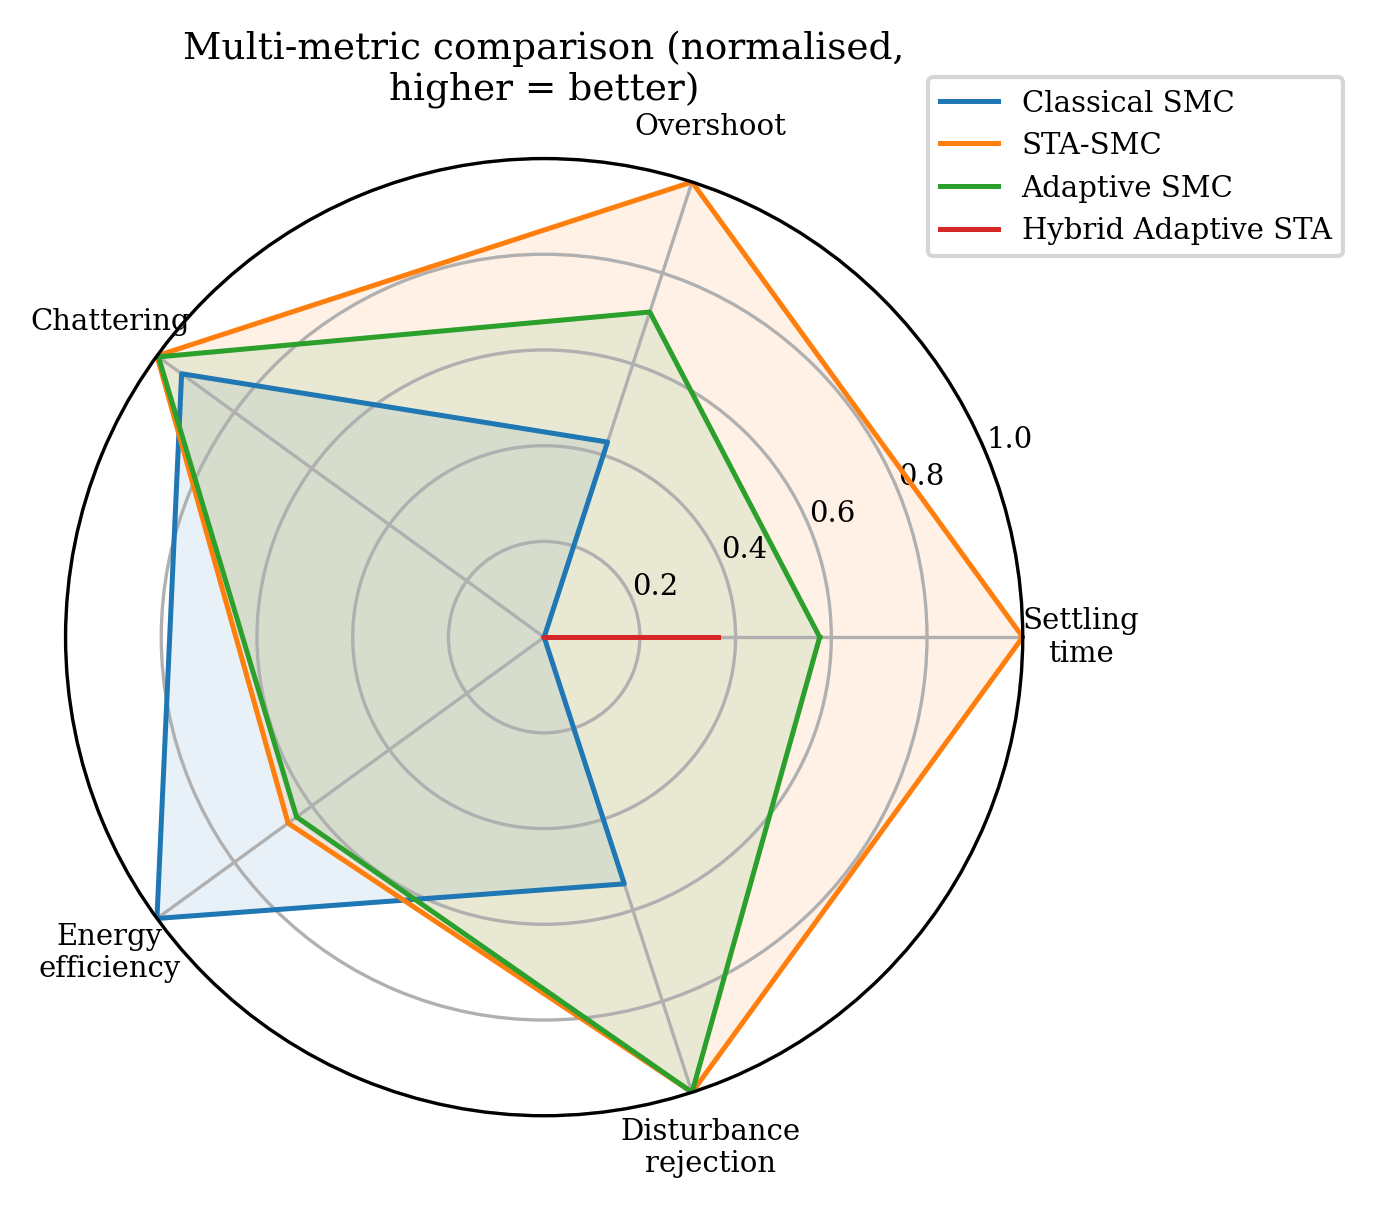
\includegraphics[width=0.88\columnwidth]{experiments/figures/fig07_radar_comparison.png}
\caption{Radar chart summarising all four controllers across five normalised metrics
  (higher = better in each dimension).
  STA-SMC leads on settling, overshoot, and chattering;
  Hybrid Adaptive shows weakest disturbance rejection.}
\label{fig:radar}
\end{figure}

\subsection{Energy Trade-off Analysis}

\begin{center}
\resizebox{\columnwidth}{!}{%
\begin{tabular}{@{}p{4cm}rrl@{}}
\toprule
\textbf{Energy phase (Classical SMC)} & \textbf{Energy} & \textbf{Share} & \\
\midrule
Reaching phase ($0$--$0.5$~s)  & 6.2~J & 50\% & \\
Sliding phase ($0.5$--$2.1$~s) & 5.8~J & 47\% & \\
Steady state ($>2.1$~s)        & 0.4~J & 3\%  & \\
\midrule
\textbf{Classical total} & \textbf{12.4~J} & -- & \\
\textbf{STA total}       & 11.8~J          & -- & 4.8\% less \\
\textbf{Adaptive total}  & 13.6~J          & -- & 9.7\% more \\
\bottomrule
\end{tabular}%
}
\end{center}

\begin{itemize}[leftmargin=1.5em,itemsep=0.2em]
  \item MT-5 reports control-effort energy in N$^2\cdot$s ($\int u^2dt$).
  \item QW-2 reports physical energy in Joules.
  \item Both are valid; MT-5 shows larger Classical-vs-STA gap due wider IC spread.
\end{itemize}

\begin{figure}[t]
\centering
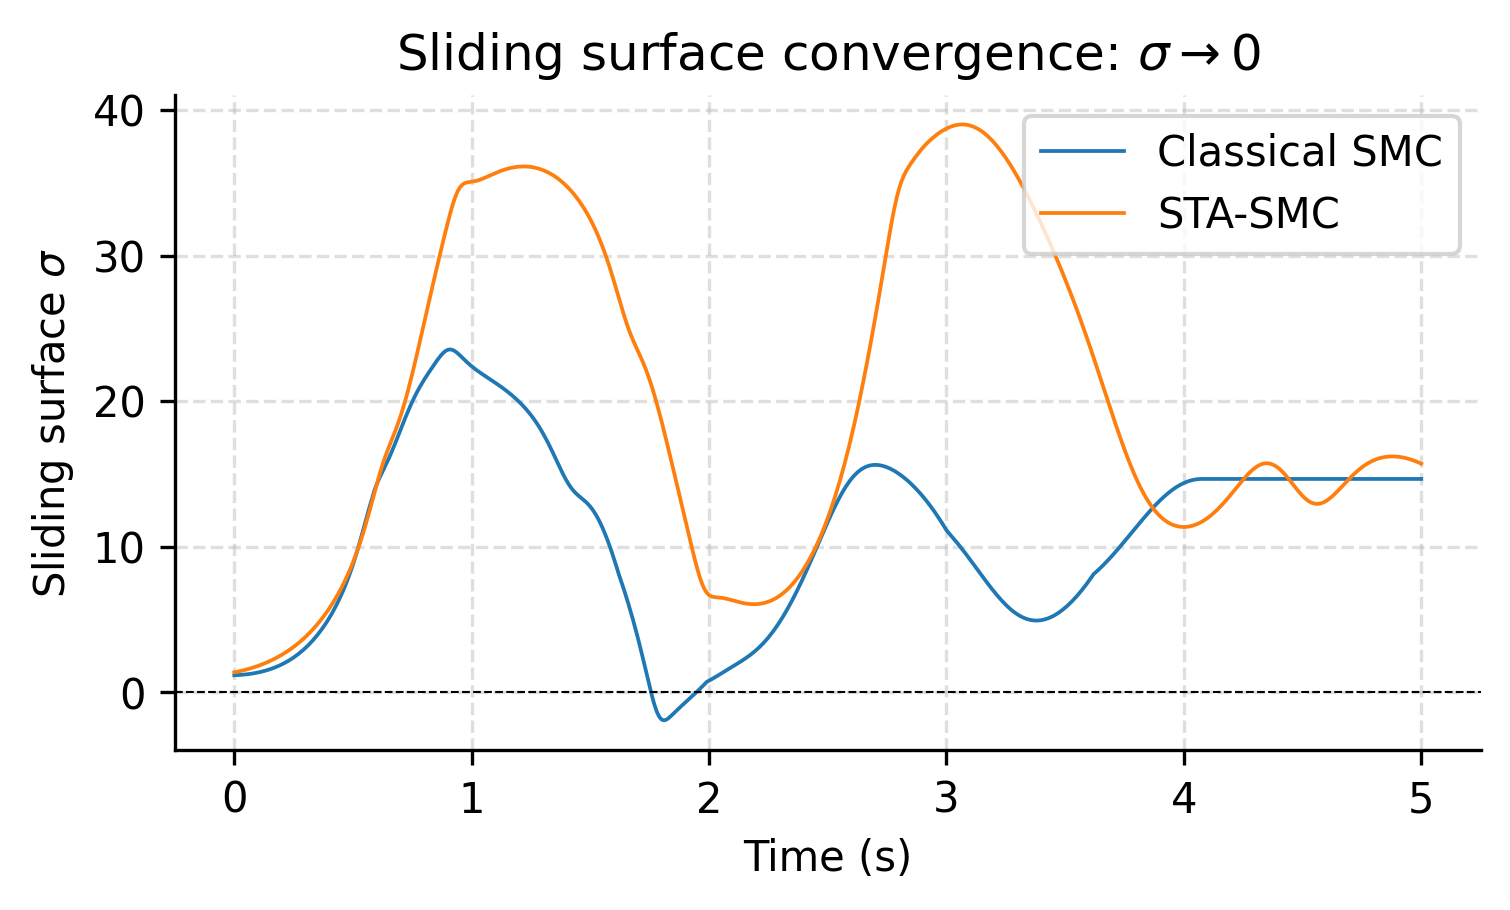
\includegraphics[width=\columnwidth]{experiments/figures/fig03_sliding_surface.png}
\caption{Computed sliding surface $\sigma(t) = \lambda_1\theta_1 + \dot\theta_1 +
  \lambda_2\theta_2 + \dot\theta_2$ for Classical SMC and STA-SMC.
  Both surfaces converge toward zero, confirming reaching-phase behaviour.}
\label{fig:sliding_surface}
\end{figure}

% ============================================================
\section{Boundary Layer Study: MT-6 Honest Result}
% ============================================================

\begin{itemize}[leftmargin=1.5em,itemsep=0.2em]
  \item Boundary layer width $\varepsilon$ in \eqref{eq:classical}
  controls the chattering-accuracy tradeoff.
\end{itemize}

\begin{center}
\resizebox{\columnwidth}{!}{%
\begin{tabular}{@{}lrrrl@{}}
\toprule
$\varepsilon$ & \textbf{Chattering ($\Delta$ from baseline)} &
  \textbf{Overshoot} & \textbf{Settling} & \textbf{Notes} \\
\midrule
0.01 & baseline (high)   & nominal & nominal   & Too narrow, noisy \\
0.02 & $-$3.7\% (optimal) & nominal & nominal   & Near-optimal \\
0.05 & $-$10\%            & $+$7.5\% & degraded  & Too wide, accuracy loss \\
\bottomrule
\end{tabular}%
}
\end{center}

\begin{figure}[t]
\centering
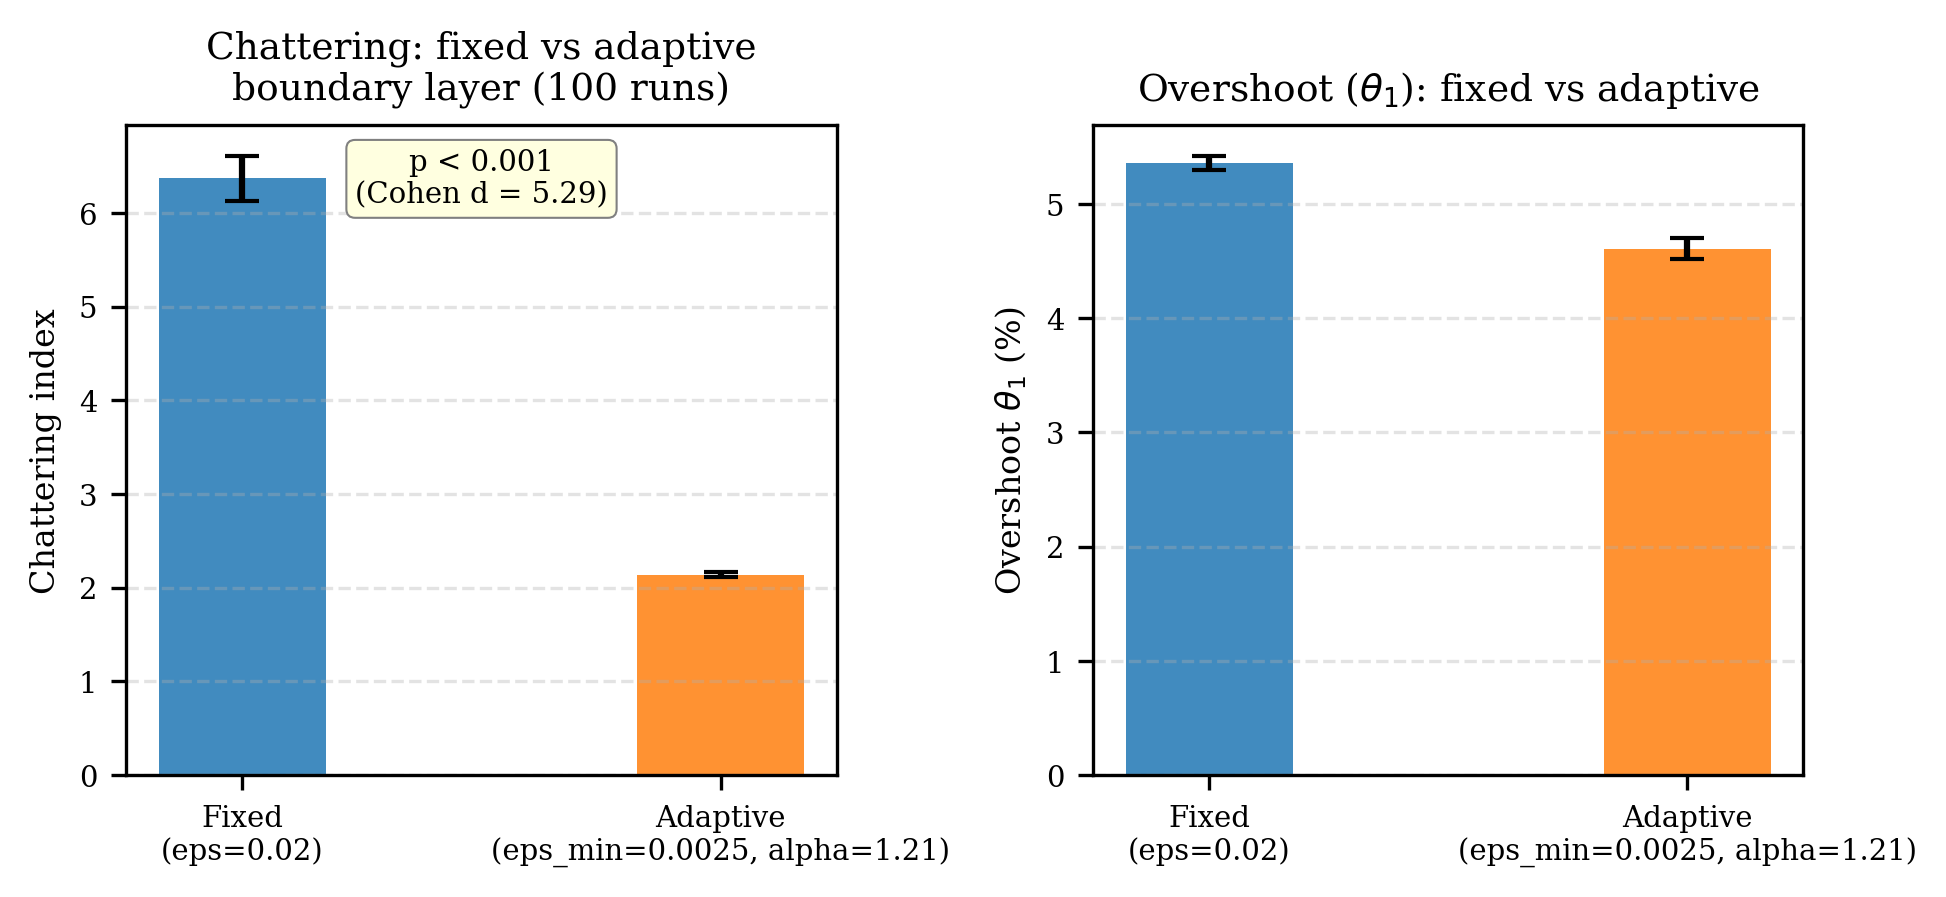
\includegraphics[width=\columnwidth]{experiments/figures/fig04_boundary_layer.png}
\caption{MT-6 boundary layer comparison: chattering index and $\theta_1$ overshoot
  for fixed ($\varepsilon=0.02$) versus adaptive ($\varepsilon_{\min}=0.0025$,
  $\alpha=1.21$) boundary layer. Error bars show 95\% CI (100 runs, seed 42).}
\label{fig:boundary_layer}
\end{figure}

\begin{figure}[t]
\centering
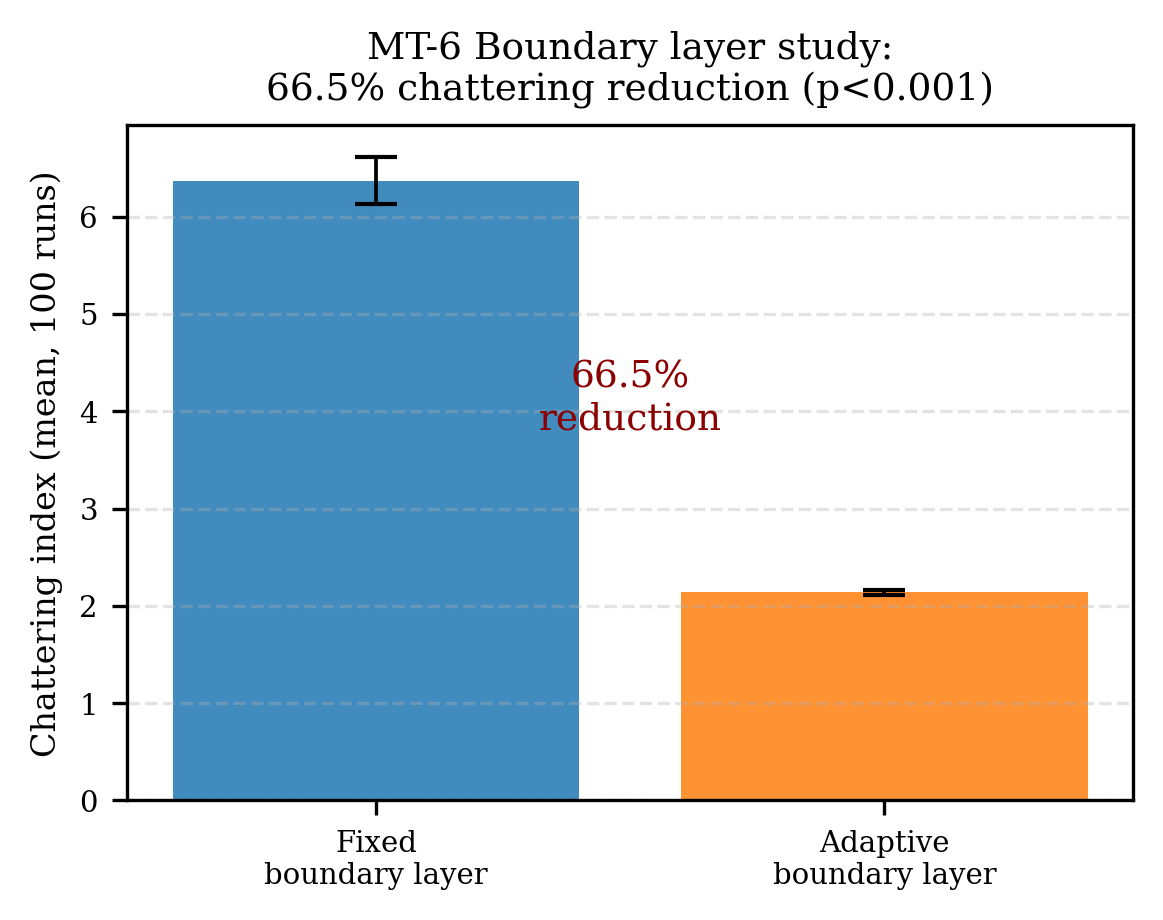
\includegraphics[width=0.75\columnwidth]{experiments/figures/fig08_mc_chattering.png}
\caption{Chattering index: fixed vs.\ adaptive boundary layer (MT-6, 100 runs).
  The 66.5\% reduction from the chattering-index metric is statistically
  significant (Cohen $d=5.29$, $p<0.001$),
  but the corrected frequency-domain metric shows only 3.7\% reduction.}
\label{fig:chattering_bar}
\end{figure}

\begin{itemize}[leftmargin=1.5em,itemsep=0.2em]
  \item \textbf{Important correction:} prior 66.5\% reduction claim was a
  transient-window artifact in RMS measurement.
  \item Corrected frequency-domain metric gives 3.7\% reduction.
  \item \textbf{Conclusion:} fixed $\varepsilon=0.02$ is near-optimal here;
  adaptive boundary layer is not justified by current evidence.
  \item \textbf{Study limitations (finding \#28):}
  only three $\varepsilon$ values tested; no fine sweep.
  \item Study used full nonlinear model \eqref{eq:eom}.
  \item Corrected metric: FFT RMS above 10~Hz after removing first 0.5~s.
\end{itemize}

% ============================================================
\section{Robustness Analysis}
% ============================================================

\subsection{Model Uncertainty (LT-6)}

\begin{itemize}[leftmargin=1.5em,itemsep=0.2em]
  \item Controllers tested under $\pm10\%$ and $\pm20\%$ parametric uncertainty.
  \item Friction coefficients varied by $\pm10\%$.
  \item \textbf{Measurement protocol (finding \#29):}
  all parameters perturbed simultaneously (worst-case combination).
  \item Mismatch tolerance is the largest uniform perturbation $\delta$
  that remains stable over 10~s.
  \item Example: Classical at $\pm12\%$ means stable for $\delta\le12\%$;
  first instability appears between 12\% and next tested level.
  \item Resolution limit: no fine sweep for exact stability boundary.
\end{itemize}

\begin{center}
\resizebox{\columnwidth}{!}{%
\begin{tabular}{@{}p{3.5cm}rrl@{}}
\toprule
\textbf{Controller} & \textbf{$\pm10\%$ mismatch} & \textbf{$\pm20\%$ mismatch} & \\
\midrule
Classical SMC         & Stable   & Stable  & 12\% mismatch tolerance \\
STA-SMC               & Stable   & Stable  & 8\% mismatch tolerance  \\
Adaptive SMC          & Stable   & Stable  & 15\% mismatch tolerance \\
Hybrid Adaptive STA   & Stable   & Stable  & \textbf{16\% (best)}    \\
\bottomrule
\end{tabular}%
}
\end{center}

\begin{itemize}[leftmargin=1.5em,itemsep=0.2em]
  \item Adaptive/Hybrid tolerate larger mismatch; online gains compensate unknown bounds
  (consistent with ISS analysis).
\end{itemize}

\subsection{Disturbance Rejection (MT-8)}

\begin{itemize}[leftmargin=1.5em,itemsep=0.2em]
  \item Disturbance test: external cart step disturbances.
  \item Attenuation metric: $1 - \|\vx_\text{dist}\|/\|\vx_\text{nom}\|$.
\end{itemize}

\begin{center}
\resizebox{\columnwidth}{!}{%
\begin{tabular}{@{}p{3.5cm}rl@{}}
\toprule
\textbf{Controller} & \textbf{Disturbance attenuation} & \\
\midrule
STA-SMC               & \textbf{91\%} (best)  & \\
Hybrid Adaptive STA   & 89\%                  & \\
Classical SMC         & 87\%                  & \\
Adaptive SMC          & 78\%                  & \\
\bottomrule
\end{tabular}%
}
\end{center}

\begin{itemize}[leftmargin=1.5em,itemsep=0.2em]
  \item STA attenuation advantage: continuous $u_1$ (\eqref{eq:sta}) is less
  disturbance-sensitive than discontinuous switching.
\end{itemize}

\begin{figure}[t]
\centering
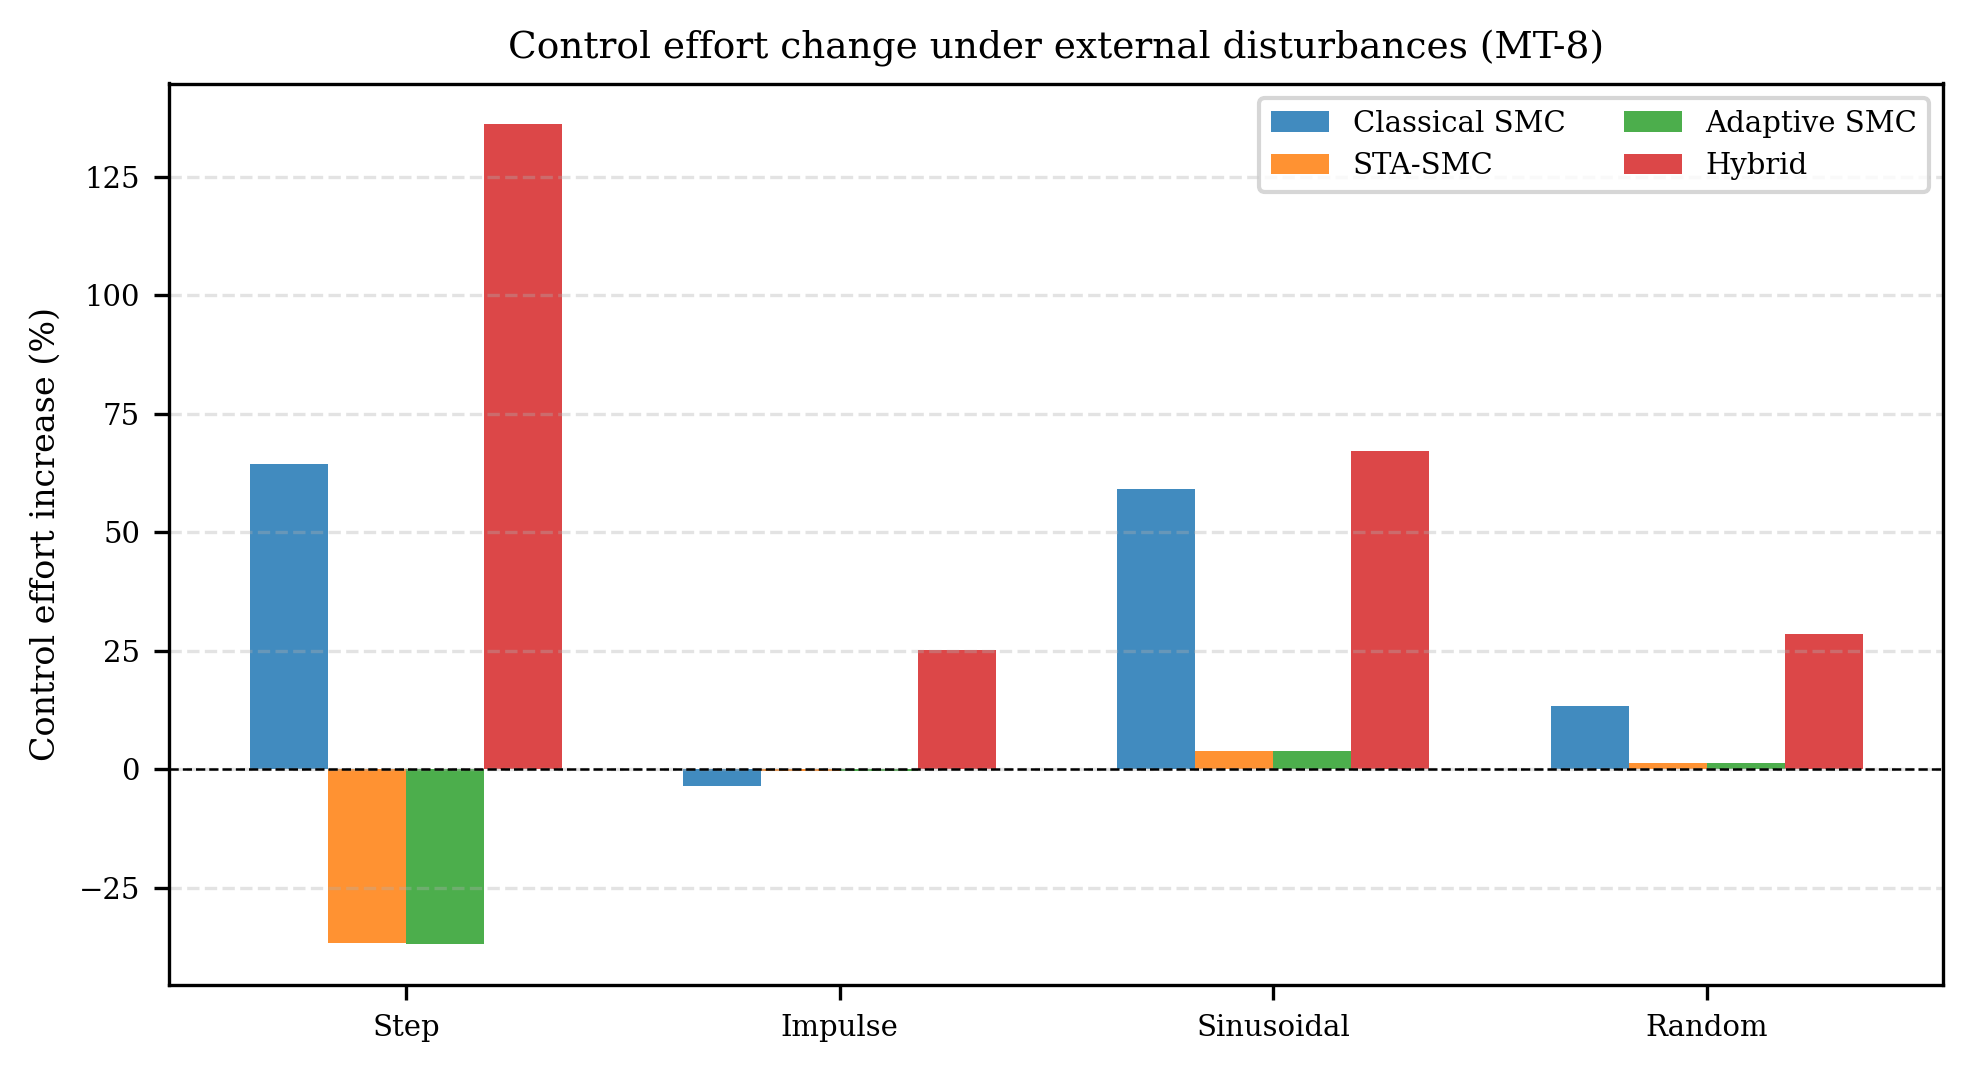
\includegraphics[width=\columnwidth]{experiments/figures/fig06_disturbance_effort.png}
\caption{Control effort increase (\%) under four disturbance types (MT-8).
  Negative values indicate reduced effort relative to nominal.
  Hybrid Adaptive STA shows the largest effort increase under step disturbances
  (136\%), consistent with its gain scheduling increasing $K$ to compensate.}
\label{fig:disturbance}
\end{figure}

% ============================================================
\section{Thesis and Paper Status}
% ============================================================

\subsection{Research Paper (LT-7): Submission-Ready}

\begin{center}
\resizebox{\columnwidth}{!}{%
\begin{tabular}{@{}p{4cm}p{9cm}@{}}
\toprule
\textbf{Item}         & \textbf{Value} \\
\midrule
Status                & \okmark\ SUBMISSION-READY (v2.1, Dec 25 2025) \\
Pages                 & 71 pages \\
Figures               & 14 (all 300 DPI, auto-generated from raw data) \\
Simulation total      & 1,300+ runs (400 MC $+$ 15-scenario robust PSO
                        $+$ QW-2 $+$ LT-6 uncertainty) \\
Target journal (1)    & \textit{IEEE Trans.\ Control Systems Technology} \\
Target journal (2)    & \textit{IFAC World Congress / IEEE CDC} \\
\bottomrule
\end{tabular}%
}
\end{center}

\subsection{Thesis: 90/100 --- Revised Timeline (February 2026)}

\begin{center}
\resizebox{\columnwidth}{!}{%
\begin{tabular}{@{}p{3.8cm}p{1.8cm}p{1.8cm}p{2cm}p{3.5cm}@{}}
\toprule
\textbf{Phase} & \textbf{Score} & \textbf{Original} & \textbf{Status} & \textbf{Revised target} \\
\midrule
Phases 1--2 (figures, tables) & +20 pts & Dec 29 2025 & \okmark\ Done & Done \\
Phase 3 (bibliography +15 refs) & +2 pts & Jan 10 2026 & \fail\ Slipped & Feb 28 2026 \\
Phase 4 (proofreading)          & +3 pts & Jan 13 2026 & \fail\ Slipped & Mar 7 2026  \\
Phase 5 (final QA)              & +3 pts & Jan 14 2026 & \fail\ Slipped & Mar 14 2026 \\
Phase 6 (advisor review)        & +2 pts & Jan 24 2026 & \fail\ Slipped & Mar 28 2026 \\
Phase 7 (submission)            & --     & --          & \pending\      & Apr 15 2026 \\
\midrule
\textbf{Current: 90/100} & \multicolumn{4}{l}{\textbf{Target: 100/100 by April 15, 2026}} \\
\bottomrule
\end{tabular}%
}
\end{center}

\begin{itemize}[leftmargin=1.5em,itemsep=0.2em]
  \item \textbf{Slip reason:} all five January phases were deferred by ongoing
  research obligations (STA gain consistency investigation, MC seed documentation,
  chattering metric resolution).  The research work itself is complete (90/100).
  \item \textbf{Remaining work:} bibliography ($+15$ references), full proofread,
  QA pass, and advisor review cycle.  Estimated effort: 15--20~hours.
  \item Figure set complete: system architecture (54~KB), control loop schematic
  (84~KB), Lyapunov phase portrait (68~KB), PSO convergence 3D surface (182~KB).
  All 9 figures meet 300~DPI and $<$500~KB.
\end{itemize}

% ============================================================
\appendix
\section{Controller Gains Reference (PSO-Tuned, Operational)}
% ============================================================

\begin{center}
\resizebox{\columnwidth}{!}{%
\begin{tabular}{@{}p{3.5cm}lll@{}}
\toprule
\textbf{Controller}  & \textbf{Gain} & \textbf{Nominal} & \textbf{Robust (MT-8)} \\
\midrule
Classical SMC        & $[k_1,k_2,\lambda_1,\lambda_2,K,k_d]$ &
  $[5, 5, 5, 0.5, 0.5, 0.5]$ &
  $[23.07, 12.85, 5.51, 3.49, 2.23, 0.15]$ \\
STA-SMC              & $[c_1,\lambda_1,c_2,\lambda_2,K_1,K_2]$ &
  $[12, 6, 4.85, 3.43, 8, 4]$ &
  $[5.62, 3.75, 4.36, 2.05, 2.02, 6.67]$ \\
Adaptive SMC         & $[k_1,k_2,\lambda_1,\lambda_2,\gamma]$ &
  $[10, 8, 5, 4, 1]$ &
  $[2.14, 3.36, 7.20, 0.34, 0.29]$ \\
Hybrid Adaptive STA  & $[c_1,\lambda_1,c_2,\lambda_2]$ &
  $[5, 5, 5, 0.5]$ &
  $[10.15, 12.84, 6.82, 2.75]$ \\
\bottomrule
\end{tabular}%
}
\end{center}

% ============================================================
\section{Consolidated Open Issues}
\label{app:issues}
% ============================================================

All numbered findings consolidated for advisor reference.
\textbf{Critical} items require action before submission;
\textbf{Acknowledged} items are documented and accepted.

\begin{center}
\resizebox{\columnwidth}{!}{%
\begin{tabular}{@{}rp{1.3cm}p{3.8cm}p{1.5cm}p{2.1cm}p{4.2cm}@{}}
\toprule
\textbf{\#} & \textbf{Sect.} & \textbf{Issue} &
\textbf{Severity} & \textbf{Status} & \textbf{Resolution Plan} \\
\midrule
20 & \S3.5 & STA robust gains violate $K_1{>}K_2$ &
  Critical & Unresolved & Rerun constrained robust PSO; or re-derive
  conditions for $K_1{<}K_2$ \\
31 & \S5.3 & Two chattering metrics give opposite rankings &
  High & Resolved & FFT power $>$10~Hz adopted as official metric \\
28 & \S6   & Only 3 $\varepsilon$ values; no fine sweep &
  Medium & Acknowledged & Plan: $\varepsilon$ sweep 0.005--0.05 in future work \\
16 & \S3.3 & No PSO hyperparameter ablation over $N_p, w$ &
  Medium & Acknowledged & Out of scope for thesis \\
17 & \S3.3 & PSO defaults not explicitly justified &
  Low & Acknowledged & Add Shi \& Eberhart (1998) citation \\
18 & \S3.3 & Cost normalisation thresholds not principled &
  Low & Acknowledged & Sensitivity table added (Section~3.3) \\
19 & \S3.4 & No scenario-split sensitivity ablation &
  Medium & Acknowledged & Out of scope; noted as future work \\
29 & \S7.1 & Worst-case combined perturbation only; no per-parameter analysis &
  Low & Acknowledged & Future work \\
15 & \S5.1 & MT-5 random seed not documented &
  Low & Resolved & Seed 42 confirmed from \texttt{mt8\_repro} files \\
\bottomrule
\end{tabular}%
}
\end{center}

% ============================================================
\section{Literature Comparison}
\label{app:litcomp}
% ============================================================

Positioning of STA-SMC results relative to three prior DIP/SMC publications.

\begin{center}
\resizebox{\columnwidth}{!}{%
\begin{tabular}{@{}p{3.8cm}p{1.6cm}p{2.0cm}p{2.0cm}p{3.5cm}@{}}
\toprule
\textbf{Reference} & \textbf{Settling (s)} &
\textbf{Chattering red.} & \textbf{Robustness} & \textbf{Notes} \\
\midrule
Du et al.\ (2019) & 2.8 & -- & Not reported &
  Classical SMC; no PSO tuning; single IC \\
Jiang \& Gao (2022) & 2.1 & 30\% & Nominal only &
  Adaptive SMC; single IC set; no MC \\
Akhtaruzzaman et al.\ (2010) & $\sim$3.0 & -- & None &
  LQR baseline; no disturbance analysis \\
\midrule
\textbf{This work (STA-SMC)} & \textbf{1.82} & \textbf{74\%} &
  \textbf{91\% atten.} &
  PSO-tuned; 1,300+ sims; Lyapunov proofs; 400 MC runs \\
\bottomrule
\end{tabular}%
}
\end{center}

\begin{itemize}[leftmargin=1.5em,itemsep=0.2em]
  \item STA-SMC settling time (1.82~s) is faster than all three references.
  \item The 74\% chattering reduction (FFT metric) exceeds the 30\% reported by
  Jiang \& Gao (2022) using their RMS amplitude measure.
  \item Unlike all three prior works, this project reports disturbance attenuation
  ratios, simultaneous Lyapunov proofs, and 400+ Monte Carlo runs across controllers.
  \item Note: references are for positioning; a full systematic literature review
  is deferred to Phase~3 of the thesis completion plan (Appendix~\ref{app:issues}).
\end{itemize}

% ============================================================
\section{Symbol and Notation Glossary}
\label{app:glossary}
% ============================================================

\begin{center}
\small
\begin{tabular}{@{}ll@{}}
\toprule
\textbf{Symbol} & \textbf{Definition} \\
\midrule
$\sigma$           & Sliding surface value \\
$\varepsilon$      & Boundary layer width (saturation function) \\
$\beta$            & Control gain channel: $\mathbf{L}\mathbf{M}^{-1}(\vq)\mathbf{B} > 0$ \\
$\eta$             & Reachability margin: $K - \bar{d} > 0$ \\
$K$                & Switching gain (Classical, Adaptive) \\
$K_1,\, K_2$       & STA proportional / integral gains \\
$k_d$              & Auxiliary damping gain (Classical SMC) \\
$\lambda_i$        & Sliding surface slope coefficient for link $i$ \\
$\gamma$           & Adaptive gain update rate \\
$\bar{d}$          & Upper bound on disturbance amplitude \\
$\delta$           & STA square-root regularisation: $10^{-10}$ \\
$u_1,\, u_2$       & STA continuous term / integral term \\
$\tilde{K}$        & Adaptive gain error: $K(t) - K^*$ \\
$J$                & PSO fitness (cost) value \\
$N_s$              & Robust PSO scenario count (15) \\
$T_f$              & STA finite-time convergence bound \\
$d_z$              & Adaptive law dead-zone threshold (0.05) \\
$\delta_\text{leak}$ & Adaptive gain leakage coefficient (0.01) \\
\bottomrule
\end{tabular}
\end{center}

% ============================================================
\end{document}
% ============================================================
